% Options for packages loaded elsewhere
% Options for packages loaded elsewhere
\PassOptionsToPackage{unicode}{hyperref}
\PassOptionsToPackage{hyphens}{url}
\PassOptionsToPackage{dvipsnames,svgnames,x11names}{xcolor}
%
\documentclass[
  letterpaper,
  DIV=11,
  numbers=noendperiod]{scrreprt}
\usepackage{xcolor}
\usepackage{amsmath,amssymb}
\setcounter{secnumdepth}{5}
\usepackage{iftex}
\ifPDFTeX
  \usepackage[T1]{fontenc}
  \usepackage[utf8]{inputenc}
  \usepackage{textcomp} % provide euro and other symbols
\else % if luatex or xetex
  \usepackage{unicode-math} % this also loads fontspec
  \defaultfontfeatures{Scale=MatchLowercase}
  \defaultfontfeatures[\rmfamily]{Ligatures=TeX,Scale=1}
\fi
\usepackage{lmodern}
\ifPDFTeX\else
  % xetex/luatex font selection
\fi
% Use upquote if available, for straight quotes in verbatim environments
\IfFileExists{upquote.sty}{\usepackage{upquote}}{}
\IfFileExists{microtype.sty}{% use microtype if available
  \usepackage[]{microtype}
  \UseMicrotypeSet[protrusion]{basicmath} % disable protrusion for tt fonts
}{}
\makeatletter
\@ifundefined{KOMAClassName}{% if non-KOMA class
  \IfFileExists{parskip.sty}{%
    \usepackage{parskip}
  }{% else
    \setlength{\parindent}{0pt}
    \setlength{\parskip}{6pt plus 2pt minus 1pt}}
}{% if KOMA class
  \KOMAoptions{parskip=half}}
\makeatother
% Make \paragraph and \subparagraph free-standing
\makeatletter
\ifx\paragraph\undefined\else
  \let\oldparagraph\paragraph
  \renewcommand{\paragraph}{
    \@ifstar
      \xxxParagraphStar
      \xxxParagraphNoStar
  }
  \newcommand{\xxxParagraphStar}[1]{\oldparagraph*{#1}\mbox{}}
  \newcommand{\xxxParagraphNoStar}[1]{\oldparagraph{#1}\mbox{}}
\fi
\ifx\subparagraph\undefined\else
  \let\oldsubparagraph\subparagraph
  \renewcommand{\subparagraph}{
    \@ifstar
      \xxxSubParagraphStar
      \xxxSubParagraphNoStar
  }
  \newcommand{\xxxSubParagraphStar}[1]{\oldsubparagraph*{#1}\mbox{}}
  \newcommand{\xxxSubParagraphNoStar}[1]{\oldsubparagraph{#1}\mbox{}}
\fi
\makeatother

\usepackage{color}
\usepackage{fancyvrb}
\newcommand{\VerbBar}{|}
\newcommand{\VERB}{\Verb[commandchars=\\\{\}]}
\DefineVerbatimEnvironment{Highlighting}{Verbatim}{commandchars=\\\{\}}
% Add ',fontsize=\small' for more characters per line
\usepackage{framed}
\definecolor{shadecolor}{RGB}{241,243,245}
\newenvironment{Shaded}{\begin{snugshade}}{\end{snugshade}}
\newcommand{\AlertTok}[1]{\textcolor[rgb]{0.68,0.00,0.00}{#1}}
\newcommand{\AnnotationTok}[1]{\textcolor[rgb]{0.37,0.37,0.37}{#1}}
\newcommand{\AttributeTok}[1]{\textcolor[rgb]{0.40,0.45,0.13}{#1}}
\newcommand{\BaseNTok}[1]{\textcolor[rgb]{0.68,0.00,0.00}{#1}}
\newcommand{\BuiltInTok}[1]{\textcolor[rgb]{0.00,0.23,0.31}{#1}}
\newcommand{\CharTok}[1]{\textcolor[rgb]{0.13,0.47,0.30}{#1}}
\newcommand{\CommentTok}[1]{\textcolor[rgb]{0.37,0.37,0.37}{#1}}
\newcommand{\CommentVarTok}[1]{\textcolor[rgb]{0.37,0.37,0.37}{\textit{#1}}}
\newcommand{\ConstantTok}[1]{\textcolor[rgb]{0.56,0.35,0.01}{#1}}
\newcommand{\ControlFlowTok}[1]{\textcolor[rgb]{0.00,0.23,0.31}{\textbf{#1}}}
\newcommand{\DataTypeTok}[1]{\textcolor[rgb]{0.68,0.00,0.00}{#1}}
\newcommand{\DecValTok}[1]{\textcolor[rgb]{0.68,0.00,0.00}{#1}}
\newcommand{\DocumentationTok}[1]{\textcolor[rgb]{0.37,0.37,0.37}{\textit{#1}}}
\newcommand{\ErrorTok}[1]{\textcolor[rgb]{0.68,0.00,0.00}{#1}}
\newcommand{\ExtensionTok}[1]{\textcolor[rgb]{0.00,0.23,0.31}{#1}}
\newcommand{\FloatTok}[1]{\textcolor[rgb]{0.68,0.00,0.00}{#1}}
\newcommand{\FunctionTok}[1]{\textcolor[rgb]{0.28,0.35,0.67}{#1}}
\newcommand{\ImportTok}[1]{\textcolor[rgb]{0.00,0.46,0.62}{#1}}
\newcommand{\InformationTok}[1]{\textcolor[rgb]{0.37,0.37,0.37}{#1}}
\newcommand{\KeywordTok}[1]{\textcolor[rgb]{0.00,0.23,0.31}{\textbf{#1}}}
\newcommand{\NormalTok}[1]{\textcolor[rgb]{0.00,0.23,0.31}{#1}}
\newcommand{\OperatorTok}[1]{\textcolor[rgb]{0.37,0.37,0.37}{#1}}
\newcommand{\OtherTok}[1]{\textcolor[rgb]{0.00,0.23,0.31}{#1}}
\newcommand{\PreprocessorTok}[1]{\textcolor[rgb]{0.68,0.00,0.00}{#1}}
\newcommand{\RegionMarkerTok}[1]{\textcolor[rgb]{0.00,0.23,0.31}{#1}}
\newcommand{\SpecialCharTok}[1]{\textcolor[rgb]{0.37,0.37,0.37}{#1}}
\newcommand{\SpecialStringTok}[1]{\textcolor[rgb]{0.13,0.47,0.30}{#1}}
\newcommand{\StringTok}[1]{\textcolor[rgb]{0.13,0.47,0.30}{#1}}
\newcommand{\VariableTok}[1]{\textcolor[rgb]{0.07,0.07,0.07}{#1}}
\newcommand{\VerbatimStringTok}[1]{\textcolor[rgb]{0.13,0.47,0.30}{#1}}
\newcommand{\WarningTok}[1]{\textcolor[rgb]{0.37,0.37,0.37}{\textit{#1}}}

\usepackage{longtable,booktabs,array}
\usepackage{calc} % for calculating minipage widths
% Correct order of tables after \paragraph or \subparagraph
\usepackage{etoolbox}
\makeatletter
\patchcmd\longtable{\par}{\if@noskipsec\mbox{}\fi\par}{}{}
\makeatother
% Allow footnotes in longtable head/foot
\IfFileExists{footnotehyper.sty}{\usepackage{footnotehyper}}{\usepackage{footnote}}
\makesavenoteenv{longtable}
\usepackage{graphicx}
\makeatletter
\newsavebox\pandoc@box
\newcommand*\pandocbounded[1]{% scales image to fit in text height/width
  \sbox\pandoc@box{#1}%
  \Gscale@div\@tempa{\textheight}{\dimexpr\ht\pandoc@box+\dp\pandoc@box\relax}%
  \Gscale@div\@tempb{\linewidth}{\wd\pandoc@box}%
  \ifdim\@tempb\p@<\@tempa\p@\let\@tempa\@tempb\fi% select the smaller of both
  \ifdim\@tempa\p@<\p@\scalebox{\@tempa}{\usebox\pandoc@box}%
  \else\usebox{\pandoc@box}%
  \fi%
}
% Set default figure placement to htbp
\def\fps@figure{htbp}
\makeatother





\setlength{\emergencystretch}{3em} % prevent overfull lines

\providecommand{\tightlist}{%
  \setlength{\itemsep}{0pt}\setlength{\parskip}{0pt}}



 


\KOMAoption{captions}{tableheading}
\makeatletter
\@ifpackageloaded{tcolorbox}{}{\usepackage[skins,breakable]{tcolorbox}}
\@ifpackageloaded{fontawesome5}{}{\usepackage{fontawesome5}}
\definecolor{quarto-callout-color}{HTML}{909090}
\definecolor{quarto-callout-note-color}{HTML}{0758E5}
\definecolor{quarto-callout-important-color}{HTML}{CC1914}
\definecolor{quarto-callout-warning-color}{HTML}{EB9113}
\definecolor{quarto-callout-tip-color}{HTML}{00A047}
\definecolor{quarto-callout-caution-color}{HTML}{FC5300}
\definecolor{quarto-callout-color-frame}{HTML}{acacac}
\definecolor{quarto-callout-note-color-frame}{HTML}{4582ec}
\definecolor{quarto-callout-important-color-frame}{HTML}{d9534f}
\definecolor{quarto-callout-warning-color-frame}{HTML}{f0ad4e}
\definecolor{quarto-callout-tip-color-frame}{HTML}{02b875}
\definecolor{quarto-callout-caution-color-frame}{HTML}{fd7e14}
\makeatother
\makeatletter
\@ifpackageloaded{bookmark}{}{\usepackage{bookmark}}
\makeatother
\makeatletter
\@ifpackageloaded{caption}{}{\usepackage{caption}}
\AtBeginDocument{%
\ifdefined\contentsname
  \renewcommand*\contentsname{Table of contents}
\else
  \newcommand\contentsname{Table of contents}
\fi
\ifdefined\listfigurename
  \renewcommand*\listfigurename{List of Figures}
\else
  \newcommand\listfigurename{List of Figures}
\fi
\ifdefined\listtablename
  \renewcommand*\listtablename{List of Tables}
\else
  \newcommand\listtablename{List of Tables}
\fi
\ifdefined\figurename
  \renewcommand*\figurename{Figure}
\else
  \newcommand\figurename{Figure}
\fi
\ifdefined\tablename
  \renewcommand*\tablename{Table}
\else
  \newcommand\tablename{Table}
\fi
}
\@ifpackageloaded{float}{}{\usepackage{float}}
\floatstyle{ruled}
\@ifundefined{c@chapter}{\newfloat{codelisting}{h}{lop}}{\newfloat{codelisting}{h}{lop}[chapter]}
\floatname{codelisting}{Listing}
\newcommand*\listoflistings{\listof{codelisting}{List of Listings}}
\makeatother
\makeatletter
\makeatother
\makeatletter
\@ifpackageloaded{caption}{}{\usepackage{caption}}
\@ifpackageloaded{subcaption}{}{\usepackage{subcaption}}
\makeatother
\usepackage{bookmark}
\IfFileExists{xurl.sty}{\usepackage{xurl}}{} % add URL line breaks if available
\urlstyle{same}
\hypersetup{
  pdftitle={Opioid Environment Toolkit for R-Spatial},
  pdfauthor={Healthy Regions \& Policies Lab},
  colorlinks=true,
  linkcolor={blue},
  filecolor={Maroon},
  citecolor={Blue},
  urlcolor={Blue},
  pdfcreator={LaTeX via pandoc}}


\title{Opioid Environment Toolkit for R-Spatial}
\author{Healthy Regions \& Policies Lab}
\date{2025-10-16}
\begin{document}
\maketitle

\renewcommand*\contentsname{Table of contents}
{
\hypersetup{linkcolor=}
\setcounter{tocdepth}{2}
\tableofcontents
}

\bookmarksetup{startatroot}

\chapter*{Preface}\label{preface}
\addcontentsline{toc}{chapter}{Preface}

\markboth{Preface}{Preface}

This toolkit provides an \textbf{introduction to GIS and spatial
analysis} for health applications that will allow researchers, analysts,
and practitioners to support their communities with better data
analytics and visualization services.

We introduce basic spatial analytic functionalities using \textbf{open
source tools}, mainly in R, using applied examples for visualizing,
mapping, and understanding the community environment. As a project of
the Justice Community Overdose Innovation network, applications covered
consider the opioid and overdose risk environment.

The
\href{https://geodacenter.github.io/opioid-environment-toolkit/index.html}{original}
toolkit version was published in 2020. This version was updated in 2025
and will continue to be expanded through the end of 2029.

\section*{Software Basics}\label{software-basics}
\addcontentsline{toc}{section}{Software Basics}

\markright{Software Basics}

We assume a basic knowledge of R and coding languages for most sections.
For most of the tutorials in this toolkit, you'll need to have R and
RStudio downloaded and installed on your system. You should be able to
install packages, know how to find the address to a folder on your
computer system, and have very basic familiarity with R. If you are new
to R, we recommend the following
\href{https://support.posit.co/hc/en-us/articles/201141096-Getting-Started-with-R}{intro-level
tutorials} provided through
\href{https://rstudio-education.github.io/hopr/starting.html}{installation}
guides. You can also refer to this
\href{https://datacarpentry.org/r-socialsci/}{R for Social Scientists}
tutorial developed by \emph{Data Carpentry} for a refresher.

We will work with following libraries, so please be sure to install:

\begin{itemize}
\tightlist
\item
  tidyverse
\item
  sf
\item
  tmap
\item
  tidygeocoder
\item
  tidycensus
\item
  units
\end{itemize}

There are differing spatial ecosystems in R. We use the \texttt{sf}
ecosystem that is compatible with the \texttt{tidyverse}. If you need to
work between these two R spatial ecosystems, see
\href{https://github.com/r-spatial/sf/wiki/Migrating}{this guide} for a
translation of \texttt{sp} to \texttt{sf} commands.

\section*{Author Team}\label{author-team}
\addcontentsline{toc}{section}{Author Team}

\markright{Author Team}

This toolkit was developed for the
\href{https://heal.nih.gov/research/research-to-practice/jcoin}{JCOIN
Network} by Marynia Kolak, Moksha Menghaney, Qinyun Lin, and Angela Li
at the Healthy Regions \& Policies Lab as part of the Methodology and
Advanced Analytics Resource Center (MAARC). The Healthy Regions Lab is
based out the University of Illinois at Urbana-Champaign, and serves as
the Geospatial Core home of the MAARC, which is situated at the
University of Chicago.

JCOIN is part of the of the NIH HEAL Initiative. The Helping to End
Addiction Long-term Initiative, or NIH HEAL Initiative, supports a wide
range of programs to develop new or improved prevention and treatment
strategies for opioid addiction.

\section*{Acknowledgements}\label{acknowledgements}
\addcontentsline{toc}{section}{Acknowledgements}

\markright{Acknowledgements}

This research was supported by the National Institutes of Health through
the NIH HEAL Initiative under award number
\href{https://reporter.nih.gov/search/3wdLGk3ipEyheDa26AEwDA/project-details/9882805\#description}{1U2CDA050098-01}
and
\href{https://reporter.nih.gov/project-details/11129703\#description}{5UM1DA050098-03}.
The contents of this publication are solely the responsibility of the
authors and do not necessarily represent the official views of the NIH,
the NIH HEAL Initiative, or the participating sites.


\includegraphics[width=5in,height=\textheight,keepaspectratio]{img/JCOIN-logo-web.jpg}

\bookmarksetup{startatroot}

\chapter{Spatial Orientation}\label{spatial-orientation}

\section{Defining spatial data}\label{SD-spatial-data}

Spatial data refers to data that contain information about specific
locations, and the information content of the data may change with
location. In other words, ``information'' and ``location'' are two
important elements in spatial data. On some occasions, spatial data may
only include ``location.'' But without ``location,'' the data is no
longer spatial anymore. For example, a spatial data that describes the
resource distribution of Medications for Opioid Overuse Disorder (MOUDs)
must contain \emph{and enable} location information of these MOUD
resources, otherwise the data becomes a non-spatial list of those
resources.

For the purpose of this tutorial, we will only briefly introduce some
important concepts in spatial data. See \emph{Further Resources} if you
would like to learn more about these concepts.

\section{Spatial data formats}\label{SD-vector-data}

Spatial data can be stored in a text file like comma-separated value
(CSV) files. However, the text file needs to have essential location
columns with latitude and longitude to represent the coordinate location
of a spatial object. Furthermore, a CSV file with lat/long columns is
only a flat/non-spatial file, until the spatial location context is
enabled as a new spatial data format.

A common spatial data format is the shapefile, which comes from
ESRI/ArcGIS proprietary software. The shapefile file format (.shp for
short) includes a minimum of 4 files, with a common prefix and different
filename extensions \texttt{.shp}, \texttt{.shx}, \texttt{.dbf}, and
\texttt{.prj}. In order to work with the spatial data, we need all these
four components of the shapefile stored in the same directory, so that
the software (such as R) can know how to project spatial objects onto a
geographic or coordinate space (i.e., spatial location context is
enabled). Other common spatial data formats include the GeoJSON, KML,
and geopackage.

\subsection{Simple features}\label{simple-features}

\href{https://r-spatial.github.io/sf/articles/sf1.html}{Simple features}
refers to an international standard (ISO 19125-1:2004) that describes
how real-world objects, and their spatial geometries, are represented in
computers. This standard is enabled in ESRI/ArcGIS architecture, POSTGIS
(a spatial extension for PostGresSQL), the GDAL libraries that serve as
underpinnings to most GIS work, and GeoJSONs. The \texttt{sf} R ecoystem
makes simple features even more accessible within R, so that simple
feature objects in spatial data are also stored in a data frame, with
one vector/column containing geographic data (usually named ``geometry''
or ``geom'').

Why should you care about these computational components of spatial
systems architecture? Spatial analysis often requires troubleshooting,
and spatial formats can be complicated.

We recommend using the \texttt{str} function in R to familiarize
yourself with data objects as you go, and to explore the data files as
well. For example: a \texttt{shapefile} includes (at least) four
components, separating the data as a \texttt{.dbf} file and projection
information as a \texttt{.prj} file. In contrast, the \texttt{sf}
spatial file loaded in your R environment is one unified object, has the
spatial information recorded as a geometry field, and projection stored
as metadata.

\section{Spatial data types}\label{spatial-data-types}

Two common formats of spatial data are vector and raster data. Vector
data represents the world surface using \textbf{points, lines, and
polygons} whereas raster data can be satellite imagery or other
pixelated surface. The figure below demonstrates how vector and raster
data models represent geographic space differently, where points, lines,
and polygons consist of the essential basis of the vector data model.

\begin{figure}[H]

{\centering 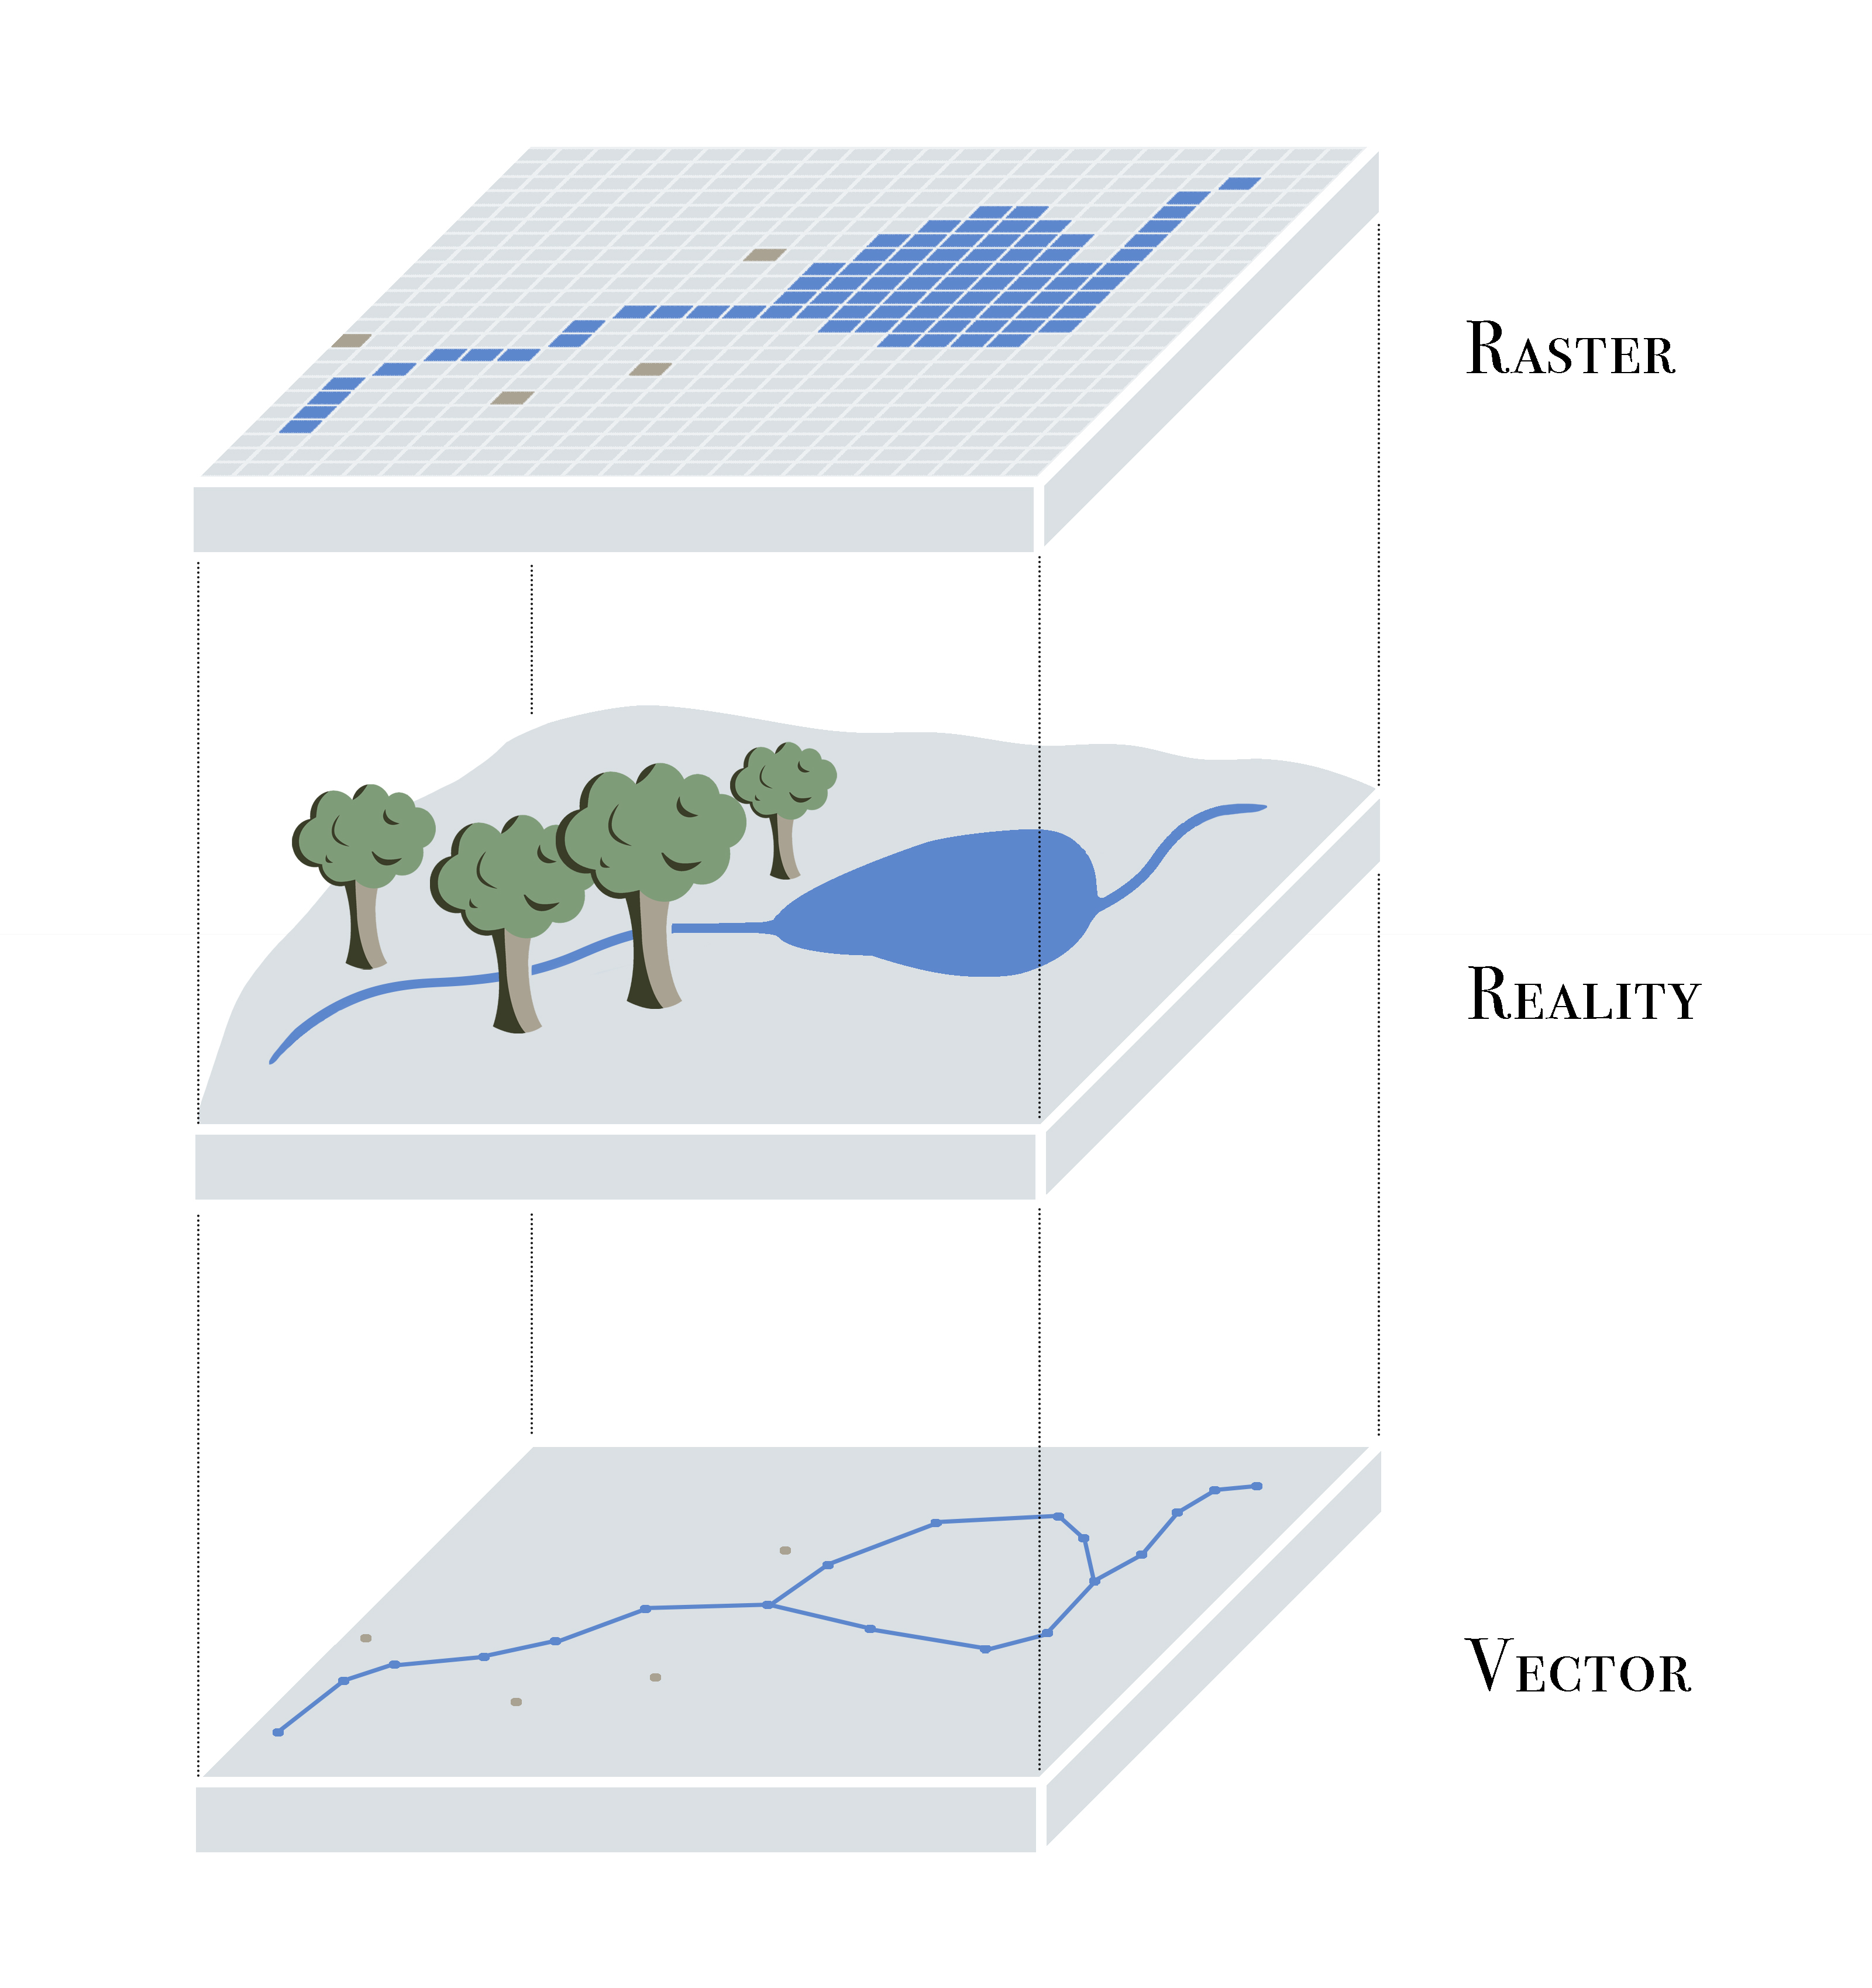
\includegraphics[width=10.67in,height=\textheight,keepaspectratio]{img/vector_raster_data_2.jpg}

}

\caption{Vector and raster data model in geographic space}

\end{figure}%

We mainly use vector data for our purpose. For example, a group of
clinics can be geocoded and converted to points, whereas zip code
boundaries are represented as polygons. Note that spatial data types
include the basic attributes \emph{in addition to} their spatial
information. So points on a map correspond to associated details for
each clinic provider, and may also include fields like ``name'',
``services'', and more. For example, each park is represented as a green
polygon in the figure below. Linked with each park, we can have
information regarding their names, sizes, types of plants, open hours,
and other various features. These attributes can be stored in a data
table, along with their spatial inforamtion, in a \texttt{shapefile}, or
a \texttt{sf} spatial file loaded in your R environment.

\begin{figure}[H]

{\centering 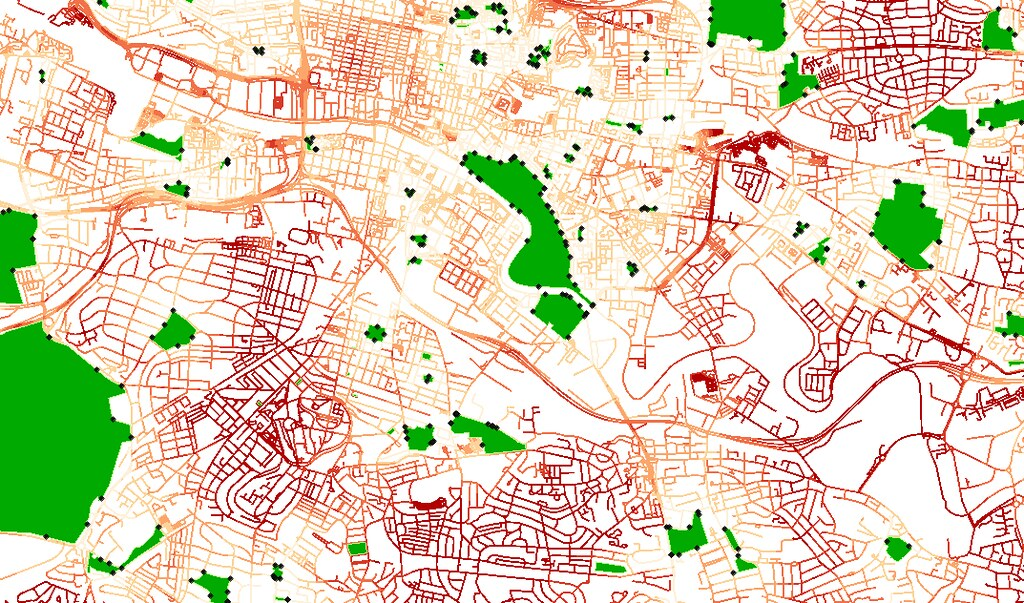
\includegraphics[width=3.41in,height=\textheight,keepaspectratio]{img/park.jpg}

}

\caption{\href{https://www.flickr.com/photos/29266908@N02/8520851663}{Glasgow
park access network} by
\href{https://www.flickr.com/photos/29266908@N02}{macrofight} is under
\href{https://creativecommons.org/licenses/by-sa/2.0/?ref=ccsearch&atype=rich}{CC
BY-SA 2.0}}

\end{figure}%

Read more regarding vector and raster data from
\href{https://geocompr.robinlovelace.net/spatial-class.html\#intro-sf}{Chapter
2 Geographic data in R} of the Lovelace et al 2019 text,
\href{https://geocompr.robinlovelace.net/}{Geocomputation with R}. This
opensource text is an incredible resource for those who are interested
in learning more details regarding geographic data analysis,
visualization, and modeling, and represents one of dozens of resources
available for learning and honing R \& spatial analysis skills.

\bookmarksetup{startatroot}

\chapter{Intro to Spatial Data}\label{intro}

\section{Overview}\label{overview}

We start our analysis with loading in our base data. Using Census tract
boundaries downloaded from the City of Chicago data portal, we'll do the
following:

\begin{itemize}
\tightlist
\item
  Read in a shapefile with the \texttt{sf} library \& convert to a
  \texttt{sf} spatial object
\item
  Inspect the spatial \emph{and} non-spatial dimensions of the data
\item
  Inspect and transform the coordinate reference system
\item
  Write the data to a new spatial data format for future use
\item
  Map the data using basics of the \texttt{tmap} library.
\end{itemize}

\section{Environment Setup}\label{BA-setup}

To replicate the code \& functions illustrated in this tutorial, you'll
need to have R and RStudio downloaded and installed on your system. This
tutorial assumes some familiarity with the R programming language.

\subsection{Input/Output}\label{BA-i-o}

Our input will be a shapefile of Chicago census tracts, as downloaded
from the City of Chicago data portal in the early 2020s. Note that at
least four files are required (.dbf, .prj, .shp, and .shx) to consitute
a shapefile.

\begin{itemize}
\tightlist
\item
  Chicago Census tracts, \texttt{Chicago\_Tracts.shp}
\end{itemize}

We will output a tract dataset geopackage (.gpkg) in a different
coordinate reference system that can be used for future analyses.

\subsection{Load Libraries}\label{load-libraries}

We will use the following packages in this tutorial:

\begin{itemize}
\tightlist
\item
  \texttt{sf}: to manipulate spatial data
\item
  \texttt{tmap}: to visualize and create maps
\end{itemize}

First, load the required libraries. \emph{Note:} You may see messages
about GEOS, GDAL, and PROJ. These refer to software libraries that allow
you to work with spatial data.

\begin{Shaded}
\begin{Highlighting}[]
\FunctionTok{library}\NormalTok{(sf)}
\end{Highlighting}
\end{Shaded}

\begin{verbatim}
Linking to GEOS 3.13.0, GDAL 3.8.5, PROJ 9.5.1; sf_use_s2() is TRUE
\end{verbatim}

\begin{Shaded}
\begin{Highlighting}[]
\FunctionTok{library}\NormalTok{(tmap)}
\end{Highlighting}
\end{Shaded}

\subsection{Load Data}\label{load-data}

First we load in the shapefile containing the census tract data
information and geographic boundaries.

\begin{Shaded}
\begin{Highlighting}[]
\NormalTok{Chi\_tracts }\OtherTok{=} \FunctionTok{st\_read}\NormalTok{(}\StringTok{"data/Chicago\_Tracts.shp"}\NormalTok{)}
\end{Highlighting}
\end{Shaded}

\begin{verbatim}
Reading layer `Chicago_Tracts' from data source 
  `/Users/maryniakolak/Code/opioid-environment-toolkit/data/Chicago_Tracts.shp' 
  using driver `ESRI Shapefile'
Simple feature collection with 801 features and 9 fields
Geometry type: POLYGON
Dimension:     XY
Bounding box:  xmin: -87.94025 ymin: 41.64429 xmax: -87.52366 ymax: 42.02392
Geodetic CRS:  WGS84(DD)
\end{verbatim}

\section{Data Inspection}\label{data-inspection}

Always inspect data when loading in.

\subsection{Non-Spatial View}\label{non-spatial-view}

First we look at a non-spatial view.

\begin{Shaded}
\begin{Highlighting}[]
\FunctionTok{head}\NormalTok{(Chi\_tracts)}
\end{Highlighting}
\end{Shaded}

\begin{verbatim}
Simple feature collection with 6 features and 9 fields
Geometry type: POLYGON
Dimension:     XY
Bounding box:  xmin: -87.68822 ymin: 41.72902 xmax: -87.62394 ymax: 41.87455
Geodetic CRS:  WGS84(DD)
  commarea commarea_n countyfp10     geoid10 name10        namelsad10 notes
1       44         44        031 17031842400   8424 Census Tract 8424  <NA>
2       59         59        031 17031840300   8403 Census Tract 8403  <NA>
3       34         34        031 17031841100   8411 Census Tract 8411  <NA>
4       31         31        031 17031841200   8412 Census Tract 8412  <NA>
5       32         32        031 17031839000   8390 Census Tract 8390  <NA>
6       28         28        031 17031838200   8382 Census Tract 8382  <NA>
  statefp10 tractce10                       geometry
1        17    842400 POLYGON ((-87.62405 41.7302...
2        17    840300 POLYGON ((-87.68608 41.8229...
3        17    841100 POLYGON ((-87.62935 41.8528...
4        17    841200 POLYGON ((-87.68813 41.8556...
5        17    839000 POLYGON ((-87.63312 41.8744...
6        17    838200 POLYGON ((-87.66782 41.8741...
\end{verbatim}

Try alternative view functions from the \texttt{tidyverse} like
glimpse().

Note the last column; this is a spatially enabled column. The data is no
longer a \texttt{shapefile} but an \texttt{sf} object, comprised of
polygons.

\subsection{Spatial View}\label{spatial-view}

We can use a \emph{baseR} function to inspect the spatial dimension. The
\texttt{sf} framework enables previews of each attribute in our spatial
file.

\begin{Shaded}
\begin{Highlighting}[]
\FunctionTok{plot}\NormalTok{(Chi\_tracts)}
\end{Highlighting}
\end{Shaded}

\pandocbounded{
\includegraphics[keepaspectratio]{intro_files/figure-pdf/spatial-view-1.pdf}}

\subsection{Structure Inspection}\label{structure-inspection}

Check out the data structure of this file\ldots{} What object is it?

\begin{Shaded}
\begin{Highlighting}[]
\FunctionTok{str}\NormalTok{(Chi\_tracts)}
\end{Highlighting}
\end{Shaded}

\begin{verbatim}
Classes 'sf' and 'data.frame':  801 obs. of  10 variables:
 $ commarea  : chr  "44" "59" "34" "31" ...
 $ commarea_n: num  44 59 34 31 32 28 65 53 76 77 ...
 $ countyfp10: chr  "031" "031" "031" "031" ...
 $ geoid10   : chr  "17031842400" "17031840300" "17031841100" "17031841200" ...
 $ name10    : chr  "8424" "8403" "8411" "8412" ...
 $ namelsad10: chr  "Census Tract 8424" "Census Tract 8403" "Census Tract 8411" "Census Tract 8412" ...
 $ notes     : chr  NA NA NA NA ...
 $ statefp10 : chr  "17" "17" "17" "17" ...
 $ tractce10 : chr  "842400" "840300" "841100" "841200" ...
 $ geometry  :sfc_POLYGON of length 801; first list element: List of 1
  ..$ : num [1:243, 1:2] -87.6 -87.6 -87.6 -87.6 -87.6 ...
  ..- attr(*, "class")= chr [1:3] "XY" "POLYGON" "sfg"
 - attr(*, "sf_column")= chr "geometry"
 - attr(*, "agr")= Factor w/ 3 levels "constant","aggregate",..: NA NA NA NA NA NA NA NA NA
  ..- attr(*, "names")= chr [1:9] "commarea" "commarea_n" "countyfp10" "geoid10" ...
\end{verbatim}

\subsection{CRS Inspection}\label{crs-inspection}

Check out the coordinate reference system. What is it? What are the
units?

\begin{Shaded}
\begin{Highlighting}[]
\FunctionTok{st\_crs}\NormalTok{(Chi\_tracts)}
\end{Highlighting}
\end{Shaded}

\begin{verbatim}
Coordinate Reference System:
  User input: WGS84(DD) 
  wkt:
GEOGCRS["WGS84(DD)",
    DATUM["WGS84",
        ELLIPSOID["WGS84",6378137,298.257223563,
            LENGTHUNIT["metre",1,
                ID["EPSG",9001]]]],
    PRIMEM["Greenwich",0,
        ANGLEUNIT["degree",0.0174532925199433]],
    CS[ellipsoidal,2],
        AXIS["longitude",east,
            ORDER[1],
            ANGLEUNIT["degree",0.0174532925199433]],
        AXIS["latitude",north,
            ORDER[2],
            ANGLEUNIT["degree",0.0174532925199433]]]
\end{verbatim}

\section{Explore Projections}\label{explore-projections}

Lets see how switching CRS changes our object. First we'll try the
Mollweide coordinate reference system that does a good job preserving
area across the globe.

\subsection{Transform CRS}\label{transform-crs}

To transform our CRS, we use the \texttt{st\_transform} function. To
plot, we use baseR again but with some parameter updates. Finally, we
check out the CRS of our new object. What are the units? Any other
details to note? Will this be appropriate for our spatial analysis?

\begin{Shaded}
\begin{Highlighting}[]
\NormalTok{Chi\_tracts.moll }\OtherTok{\textless{}{-}} \FunctionTok{st\_transform}\NormalTok{(Chi\_tracts, }\AttributeTok{crs=}\StringTok{"ESRI:54009"}\NormalTok{)}

\FunctionTok{plot}\NormalTok{(}\FunctionTok{st\_geometry}\NormalTok{(Chi\_tracts.moll), }\AttributeTok{border =} \StringTok{"gray"}\NormalTok{, }\AttributeTok{lwd =} \DecValTok{2}\NormalTok{, }\AttributeTok{main =} \StringTok{"Mollweide"}\NormalTok{, }\AttributeTok{sub=}\StringTok{"preserves areas"}\NormalTok{)}
\end{Highlighting}
\end{Shaded}

\pandocbounded{
\includegraphics[keepaspectratio]{intro_files/figure-pdf/mollweide-crs-1.pdf}}

\begin{Shaded}
\begin{Highlighting}[]
\FunctionTok{st\_crs}\NormalTok{(Chi\_tracts.moll)}
\end{Highlighting}
\end{Shaded}

\begin{verbatim}
Coordinate Reference System:
  User input: ESRI:54009 
  wkt:
PROJCRS["World_Mollweide",
    BASEGEOGCRS["WGS 84",
        DATUM["World Geodetic System 1984",
            ELLIPSOID["WGS 84",6378137,298.257223563,
                LENGTHUNIT["metre",1]]],
        PRIMEM["Greenwich",0,
            ANGLEUNIT["Degree",0.0174532925199433]]],
    CONVERSION["World_Mollweide",
        METHOD["Mollweide"],
        PARAMETER["Longitude of natural origin",0,
            ANGLEUNIT["Degree",0.0174532925199433],
            ID["EPSG",8802]],
        PARAMETER["False easting",0,
            LENGTHUNIT["metre",1],
            ID["EPSG",8806]],
        PARAMETER["False northing",0,
            LENGTHUNIT["metre",1],
            ID["EPSG",8807]]],
    CS[Cartesian,2],
        AXIS["(E)",east,
            ORDER[1],
            LENGTHUNIT["metre",1]],
        AXIS["(N)",north,
            ORDER[2],
            LENGTHUNIT["metre",1]],
    USAGE[
        SCOPE["Not known."],
        AREA["World."],
        BBOX[-90,-180,90,180]],
    ID["ESRI",54009]]
\end{verbatim}

Next, we'll try the Winkel CRS, which is a compromise projection that
facilitates minimal distortion for area, distance, and angles. We use
the same approach, recyling the code with new inputs.

\begin{Shaded}
\begin{Highlighting}[]
\NormalTok{Chi\_tracts}\FloatTok{.54019} \OtherTok{=} \FunctionTok{st\_transform}\NormalTok{(Chi\_tracts, }\AttributeTok{crs=}\StringTok{"ESRI:54019"}\NormalTok{)}
\FunctionTok{plot}\NormalTok{(}\FunctionTok{st\_geometry}\NormalTok{(Chi\_tracts}\FloatTok{.54019}\NormalTok{), }\AttributeTok{border =} \StringTok{"gray"}\NormalTok{, }\AttributeTok{lwd =} \DecValTok{2}\NormalTok{, }\AttributeTok{main =} \StringTok{"Winkel"}\NormalTok{, }\AttributeTok{sub=}\StringTok{"minimal distortion"}\NormalTok{)}
\end{Highlighting}
\end{Shaded}

\pandocbounded{
\includegraphics[keepaspectratio]{intro_files/figure-pdf/winkel-crs-1.pdf}}

\begin{Shaded}
\begin{Highlighting}[]
\FunctionTok{st\_crs}\NormalTok{(Chi\_tracts}\FloatTok{.54019}\NormalTok{)}
\end{Highlighting}
\end{Shaded}

\begin{verbatim}
Coordinate Reference System:
  User input: ESRI:54019 
  wkt:
PROJCRS["World_Winkel_II",
    BASEGEOGCRS["WGS 84",
        DATUM["World Geodetic System 1984",
            ELLIPSOID["WGS 84",6378137,298.257223563,
                LENGTHUNIT["metre",1]]],
        PRIMEM["Greenwich",0,
            ANGLEUNIT["Degree",0.0174532925199433]]],
    CONVERSION["World_Winkel_II",
        METHOD["Winkel II"],
        PARAMETER["Longitude of natural origin",0,
            ANGLEUNIT["Degree",0.0174532925199433],
            ID["EPSG",8802]],
        PARAMETER["Latitude of 1st standard parallel",50.4597762521898,
            ANGLEUNIT["Degree",0.0174532925199433],
            ID["EPSG",8823]],
        PARAMETER["False easting",0,
            LENGTHUNIT["metre",1],
            ID["EPSG",8806]],
        PARAMETER["False northing",0,
            LENGTHUNIT["metre",1],
            ID["EPSG",8807]]],
    CS[Cartesian,2],
        AXIS["(E)",east,
            ORDER[1],
            LENGTHUNIT["metre",1]],
        AXIS["(N)",north,
            ORDER[2],
            LENGTHUNIT["metre",1]],
    USAGE[
        SCOPE["Not known."],
        AREA["World."],
        BBOX[-90,-180,90,180]],
    ID["ESRI",54019]]
\end{verbatim}

We could also try a totally different projection, to see how that
changes our spatial object. Let's use the ``Old Hawaiian UTM Zone 4n''
projection, with the EPSG identified from an online search. How does
this fare?

\begin{Shaded}
\begin{Highlighting}[]
\NormalTok{Chi\_tracts.Hawaii }\OtherTok{=} \FunctionTok{st\_transform}\NormalTok{(Chi\_tracts, }\AttributeTok{crs=}\StringTok{"ESRI:102114"}\NormalTok{)}
\FunctionTok{plot}\NormalTok{(}\FunctionTok{st\_geometry}\NormalTok{(Chi\_tracts.Hawaii), }\AttributeTok{border =} \StringTok{"gray"}\NormalTok{, }\AttributeTok{lwd =} \DecValTok{2}\NormalTok{, }\AttributeTok{main =} \StringTok{"Old Hawaiian UTM Zone 4N"}\NormalTok{, }\AttributeTok{sub=}\StringTok{"wrong projection!"}\NormalTok{)}
\end{Highlighting}
\end{Shaded}

\pandocbounded{
\includegraphics[keepaspectratio]{intro_files/figure-pdf/hawaii-crs-1.pdf}}

Finally.. let's choose a projection that is focused on Illinois, and
uses distance as feet or meters, to make it a bit more accessible for
our work. EPSG:3435 is a good fit:

\begin{Shaded}
\begin{Highlighting}[]
\NormalTok{Chi\_tracts}\FloatTok{.3435} \OtherTok{\textless{}{-}} \FunctionTok{st\_transform}\NormalTok{(Chi\_tracts, }\StringTok{"EPSG:3435"}\NormalTok{)}
\CommentTok{\# Chi\_tracts.3435 \textless{}{-} st\_transform(Chi\_tracts, 3435)}
\FunctionTok{st\_crs}\NormalTok{(Chi\_tracts}\FloatTok{.3435}\NormalTok{)}
\end{Highlighting}
\end{Shaded}

\begin{verbatim}
Coordinate Reference System:
  User input: EPSG:3435 
  wkt:
PROJCRS["NAD83 / Illinois East (ftUS)",
    BASEGEOGCRS["NAD83",
        DATUM["North American Datum 1983",
            ELLIPSOID["GRS 1980",6378137,298.257222101,
                LENGTHUNIT["metre",1]]],
        PRIMEM["Greenwich",0,
            ANGLEUNIT["degree",0.0174532925199433]],
        ID["EPSG",4269]],
    CONVERSION["SPCS83 Illinois East zone (US survey foot)",
        METHOD["Transverse Mercator",
            ID["EPSG",9807]],
        PARAMETER["Latitude of natural origin",36.6666666666667,
            ANGLEUNIT["degree",0.0174532925199433],
            ID["EPSG",8801]],
        PARAMETER["Longitude of natural origin",-88.3333333333333,
            ANGLEUNIT["degree",0.0174532925199433],
            ID["EPSG",8802]],
        PARAMETER["Scale factor at natural origin",0.999975,
            SCALEUNIT["unity",1],
            ID["EPSG",8805]],
        PARAMETER["False easting",984250,
            LENGTHUNIT["US survey foot",0.304800609601219],
            ID["EPSG",8806]],
        PARAMETER["False northing",0,
            LENGTHUNIT["US survey foot",0.304800609601219],
            ID["EPSG",8807]]],
    CS[Cartesian,2],
        AXIS["easting (X)",east,
            ORDER[1],
            LENGTHUNIT["US survey foot",0.304800609601219]],
        AXIS["northing (Y)",north,
            ORDER[2],
            LENGTHUNIT["US survey foot",0.304800609601219]],
    USAGE[
        SCOPE["Engineering survey, topographic mapping."],
        AREA["United States (USA) - Illinois - counties of Boone; Champaign; Clark; Clay; Coles; Cook; Crawford; Cumberland; De Kalb; De Witt; Douglas; Du Page; Edgar; Edwards; Effingham; Fayette; Ford; Franklin; Gallatin; Grundy; Hamilton; Hardin; Iroquois; Jasper; Jefferson; Johnson; Kane; Kankakee; Kendall; La Salle; Lake; Lawrence; Livingston; Macon; Marion; Massac; McHenry; McLean; Moultrie; Piatt; Pope; Richland; Saline; Shelby; Vermilion; Wabash; Wayne; White; Will; Williamson."],
        BBOX[37.06,-89.27,42.5,-87.02]],
    ID["EPSG",3435]]
\end{verbatim}

\begin{Shaded}
\begin{Highlighting}[]
\FunctionTok{plot}\NormalTok{(}\FunctionTok{st\_geometry}\NormalTok{(Chi\_tracts}\FloatTok{.3435}\NormalTok{), }\AttributeTok{border =} \StringTok{"gray"}\NormalTok{, }\AttributeTok{lwd =} \DecValTok{2}\NormalTok{, }\AttributeTok{main =} \StringTok{"NAD83 / Illinois East (ftUS)"}\NormalTok{, }\AttributeTok{sub=}\StringTok{"topo mapping \& survey use"}\NormalTok{)}
\end{Highlighting}
\end{Shaded}

\pandocbounded{
\includegraphics[keepaspectratio]{intro_files/figure-pdf/3435-crs-1.pdf}}

\section{Write Data}\label{write-data}

We transformed our Chicago tract spatial dataset to a coordinate
reference system that is appropriate for Illinois-specific analysis,
using a distance measure that is interpretable for our purposes. Let's
write that file to our directory.

We'll write to a new, elegant spatial data format, the
\emph{geopackage}. Uncomment the line, and run.

\begin{Shaded}
\begin{Highlighting}[]
\CommentTok{\#st\_write(Chi\_tracts.3435, "data/ChiTracts{-}3435.gpkg")}
\end{Highlighting}
\end{Shaded}

Now we'll switch to a more extensive cartographic mapping package,
\texttt{tmap}, to map our data.

\section{Map the Basics}\label{map-the-basics}

We approach mapping with one layer at a time. Always start with the
object you want to map by calling it with the \texttt{tm\_shape}
function. Then, at least one descriptive/styling function follows. There
are hundreds of variations and paramater specifications, so take your
time in exploring \texttt{tmap} and the options.

Here we style the tracts with some semi-transparent borders.

\begin{Shaded}
\begin{Highlighting}[]
\FunctionTok{tm\_shape}\NormalTok{(Chi\_tracts}\FloatTok{.3435}\NormalTok{) }\SpecialCharTok{+} 
  \FunctionTok{tm\_borders}\NormalTok{(}\AttributeTok{lwd =} \FloatTok{0.5}\NormalTok{) }
\end{Highlighting}
\end{Shaded}

\pandocbounded{
\includegraphics[keepaspectratio]{intro_files/figure-pdf/unnamed-chunk-2-1.pdf}}

Next we fill the tracts with a light gray, and adjust the color and
transparency of borders. We also add a scale bar, positioning it to the
left and having a thickness of 0.8 units, and turn off the frame. See
more specifications for `tm\_polygons' at
\href{https://r-tmap.github.io/tmap/reference/tm_polygons.html?q=tm_polygons\#null}{tmap
documentations}.

\begin{Shaded}
\begin{Highlighting}[]
\FunctionTok{tm\_shape}\NormalTok{(Chi\_tracts) }\SpecialCharTok{+} 
  \FunctionTok{tm\_polygons}\NormalTok{(}
    \AttributeTok{fill =} \StringTok{"gray90"}\NormalTok{, }\CommentTok{\#fill color}
    \AttributeTok{col =} \StringTok{"gray10"}\NormalTok{, }\CommentTok{\#border color}
    \AttributeTok{lwd =} \FloatTok{0.5} \CommentTok{\#line width}
\NormalTok{    ) }\SpecialCharTok{+} 
  \FunctionTok{tm\_scalebar}\NormalTok{(}\AttributeTok{position =} \FunctionTok{c}\NormalTok{(}\StringTok{"bottom"}\NormalTok{,}\StringTok{"left"}\NormalTok{), }\AttributeTok{lwd =} \FloatTok{0.8}\NormalTok{) }\SpecialCharTok{+}
  \FunctionTok{tm\_layout}\NormalTok{(}\AttributeTok{frame =} \ConstantTok{FALSE}\NormalTok{)}
\end{Highlighting}
\end{Shaded}

\pandocbounded{
\includegraphics[keepaspectratio]{intro_files/figure-pdf/unnamed-chunk-3-1.pdf}}

Check out the \href{https://r-tmap.github.io/tmap/reference}{tmap
Reference manual} for more ideas!

\section*{More Resources}\label{more-resources}
\addcontentsline{toc}{section}{More Resources}

\markright{More Resources}

On spatial data basics \& sf:

\begin{itemize}
\item
  \url{https://r.geocompx.org/intro.html}
\item
  \url{https://geodacenter.github.io/opioid-environment-toolkit/spatial-data-introduction.html}
\end{itemize}

On projections:

\begin{itemize}
\item
  \url{https://desktop.arcgis.com/en/arcmap/10.3/guide-books/map-projections/projection-basics-for-gis-professionals.htm}
\item
  \url{https://geocompr.robinlovelace.net/reproj-geo-data.html}
\item
  \url{https://datacarpentry.org/organization-geospatial/03-crs/index.html}
\end{itemize}

On tmap:

\begin{itemize}
\item
  \url{https://cran.r-project.org/web/packages/tmap/vignettes/tmap-getstarted.html}
\item
  \url{https://geocompr.robinlovelace.net/adv-map.html}
\end{itemize}

\bookmarksetup{startatroot}

\chapter{Geocoding Locations}\label{geocode-points}

\section{Overview}\label{GA-research-question}

A common goal in opioid environment research is to calculate and compare
access metrics to different providers of Medications for Opioid Overuse
Disorder (MOUDs). Before we can run any analytics on the resource
location data, we need to convert resource addresses to spatial data
points, which can be then used to calculate access metrics.

\textbf{Geocoding} is the process of converting addresses (like a street
address) into geographic coordinates using a known coordinate reference
system. We can then use these coordinates (latitude, longitude) to
spatially enable our data. This means we convert to a spatial data frame
(sf) within R for spatial analysis within our R session, and then save
as a shapefile (a spatial data format) for future use. In this tutorial
we demonstrate how to geocode resource location addresses and convert to
spatial data points that can be used for future mapping and geospatial
analysis.

Our objectives are thus to:

\begin{itemize}
\tightlist
\item
  Geocode addresses to get geographic coordinates
\item
  Visualize the resource locations as points on a map in R
\item
  Transform a flat file (.CSV) to a spatially enabled shapefile (.SHP)
\end{itemize}

\section{Environment Setup}\label{GA-setup}

To replicate the code \& functions illustrated in this tutorial, you'll
need to have R and RStudio downloaded and installed on your system. This
tutorial assumes some familiarity with the R programming language.

\subsection{Input/Output}\label{GA-i-o}

Our input will be a \textbf{CSV} file that include addresses of our
resources. This file can be found
\href{https://github.com/GeoDaCenter/opioid-environment-toolkit/tree/master/data}{here}.

\begin{itemize}
\tightlist
\item
  Chicago Methadone Clinics, \texttt{chicago\_methadone.csv}
\end{itemize}

We will convert these addresses to geographic coordinates using an
appropriate coordinate reference system (CRS), and then spatially enable
the data for mapping. We will then export the spatial dataframe as a
\textbf{shapefile}.

\subsection{Load Libraries}\label{GA-packages1}

We will use the following packages in this tutorial:

\begin{itemize}
\tightlist
\item
  \texttt{sf}: to manipulate spatial data
\item
  \texttt{tmap}: to visualize and create maps
\item
  \texttt{tidygeocoder}: to convert addresses to geographic coordinates
\end{itemize}

Then load the libraries for use.

\begin{Shaded}
\begin{Highlighting}[]
\FunctionTok{library}\NormalTok{(sf)}
\FunctionTok{library}\NormalTok{(tidygeocoder)}
\FunctionTok{library}\NormalTok{(tmap)}
\end{Highlighting}
\end{Shaded}

\subsection{Load Data}\label{load-data-1}

We will use a CSV that includes methadone clinic addresses in Chicago as
an example. We start with a small dataset to test our geocoding
workflow, as best practice.

Let's take a look at the first few rows of the dataset. Our data
includes addresses but not geographic coordinates.

\begin{Shaded}
\begin{Highlighting}[]
\NormalTok{methadoneClinics }\OtherTok{\textless{}{-}} \FunctionTok{read.csv}\NormalTok{(}\StringTok{"data/chicago\_methadone\_nogeometry.csv"}\NormalTok{)}
\FunctionTok{head}\NormalTok{(methadoneClinics)}
\end{Highlighting}
\end{Shaded}

\begin{verbatim}
  X                                                         Name
1 1                Chicago Treatment and Counseling Center, Inc.
2 2                      Sundace Methadone Treatment Center, LLC
3 3 Soft Landing Interventions/DBA Symetria Recovery of Lakeview
4 4                                        PDSSC - Chicago, Inc.
5 5                          Center for Addictive Problems, Inc.
6 6                                Family Guidance Centers, Inc.
                  Address    City State   Zip
1 4453 North Broadway st. Chicago    IL 60640
2 4545 North Broadway St. Chicago    IL 60640
3    3934 N. Lincoln Ave. Chicago    IL 60613
4     2260 N. Elston Ave. Chicago    IL 60614
5        609 N. Wells St. Chicago    IL 60654
6     310 W. Chicago Ave. Chicago    IL 60654
\end{verbatim}

\section{Geocode addresses}\label{GA-geocode-addresses}

\subsection{Quality Control}\label{quality-control}

Before geocoding, perform an initial quality check on the data. Note
that the address, city, state, and zip code are all separated as
different columns. This will make it easier to stitch together for a
coherent, standard address for geocoding. Furthermore, there do not
appear to be any major errors. The city name ``Chicago'' is spelled
consistently, without missing addresses or zip codes. This will not
always be the case, unfortunately. Data must be cleaned prior to loading
into a geocoding service.

\subsection{Selecting Geocoding
Service}\label{selecting-geocoding-service}

To get a geographic coordinate for each site, we'll need to geocode.
There are a number of geocoding options in R; here we use we the
\texttt{tidygeocoder} package. It uses
\href{https://jessecambon.github.io/tidygeocoder/articles/geocoder_services.html}{mutliple
geocoding services}, providing the user with an option to choose. It
also provides the option to use a \texttt{osm} method which uses the
Nominatum service, allowing 1 query per second. More powerful services
are available that are even more effective for batch geocoding
(i.e.~larger volume of addresses). Many will require an API key,
necessitating registration and additional funds to purchase access in
some cases.

When considering which geocoding service to use, consider scale and
potential geocoding errors. Some geocoding services are more accurate
than others, so if your coordinates were not coded precisely, try a
different service. If you have thousands of addresses to geocode, you
may require more complex data pipelines. For an open option with no API
key required, you can try the
\href{https://geocoding.geo.census.gov/}{US Census geocoder} (or
\texttt{census} method in this package), which allows around 10,000
addresses to be geocoded at once. Others have varying daily limits.
Google Maps API and ESRI Geocoding service are additional high-quality
geocoding services with varying cost associated, both within and outside
this package.

\begin{tcolorbox}[enhanced jigsaw, title=\textcolor{quarto-callout-important-color}{\faExclamation}\hspace{0.5em}{Is your data private?}, bottomtitle=1mm, rightrule=.15mm, bottomrule=.15mm, breakable, colbacktitle=quarto-callout-important-color!10!white, opacitybacktitle=0.6, coltitle=black, toprule=.15mm, leftrule=.75mm, opacityback=0, toptitle=1mm, titlerule=0mm, colback=white, arc=.35mm, left=2mm, colframe=quarto-callout-important-color-frame]

If you are working with private data that has additional protections,
you should not use a geocoding service that is connected to the
internet. Because addresses are being passed through a web service, it
is not considered protected. That includes the geocoding services
presented in \texttt{tidygeocoder}!

For protected data, you must use a HIPAA-compliant geocoding service
that works offline. You can build one through Nominatum (see example
\href{https://mapscaping.com/open\%E2\%80\%91source-geocoding-with-nominatim-and-geopy/}{here}),
use an ESRI partner product (see example
\href{https://www.esri.com/partners/spatialitics-a2Tf20000056o9TEAQ/healthcare-geocoder-a2df2000004MiL4AAK}{here}),
or check out additional options.

\end{tcolorbox}

\subsection{Test Geocoding Service}\label{test-geocoding-service}

Before geocoding your entire dataset, first review the documentation for
the geocoding service you'll be using. In our example we use
\texttt{tidygeocoder}, with documentation found
\href{https://cran.r-project.org/web/packages/tidygeocoder/vignettes/tidygeocoder.html}{here}.
Let's test the service by starting with one address:

\begin{Shaded}
\begin{Highlighting}[]
\NormalTok{sample }\OtherTok{\textless{}{-}} \FunctionTok{geo}\NormalTok{(}\StringTok{"4545 North Broadway St. Chicago, IL"}\NormalTok{, }\AttributeTok{lat =}\NormalTok{ latitude, }\AttributeTok{long =}\NormalTok{ longitude, }\AttributeTok{method =} \StringTok{\textquotesingle{}osm\textquotesingle{}}\NormalTok{)}
\end{Highlighting}
\end{Shaded}

\begin{verbatim}
Passing 1 address to the Nominatim single address geocoder
\end{verbatim}

\begin{verbatim}
Query completed in: 1.2 seconds
\end{verbatim}

\begin{Shaded}
\begin{Highlighting}[]
\NormalTok{sample}
\end{Highlighting}
\end{Shaded}

\begin{verbatim}
# A tibble: 1 x 3
  address                             latitude longitude
  <chr>                                  <dbl>     <dbl>
1 4545 North Broadway St. Chicago, IL     42.0     -87.7
\end{verbatim}

What did the output look like? Get familiar with the input parameters,
expected output, and review the documentation further if needed.

\subsection{Prepare input parameter}\label{prepare-input-parameter}

To apply the function to multiple addresses, we first we need ensure
that we have a \emph{character vector} of full addresses.

\begin{Shaded}
\begin{Highlighting}[]
\FunctionTok{str}\NormalTok{(methadoneClinics)}
\end{Highlighting}
\end{Shaded}

\begin{verbatim}
'data.frame':   27 obs. of  6 variables:
 $ X      : int  1 2 3 4 5 6 7 8 9 10 ...
 $ Name   : chr  "Chicago Treatment and Counseling Center, Inc." "Sundace Methadone Treatment Center, LLC" "Soft Landing Interventions/DBA Symetria Recovery of Lakeview" "PDSSC - Chicago, Inc." ...
 $ Address: chr  "4453 North Broadway st." "4545 North Broadway St." "3934 N. Lincoln Ave." "2260 N. Elston Ave." ...
 $ City   : chr  "Chicago" "Chicago" "Chicago" "Chicago" ...
 $ State  : chr  "IL" "IL" "IL" "IL" ...
 $ Zip    : int  60640 60640 60613 60614 60654 60654 60651 60607 60607 60616 ...
\end{verbatim}

Next we convert all fields to character first to avoid issues with
factors (a common peril of R!).

\begin{Shaded}
\begin{Highlighting}[]
\NormalTok{methadoneClinics}\SpecialCharTok{$}\NormalTok{fullAdd }\OtherTok{\textless{}{-}} \FunctionTok{paste}\NormalTok{(}\FunctionTok{as.character}\NormalTok{(methadoneClinics}\SpecialCharTok{$}\NormalTok{Address), }
                                  \FunctionTok{as.character}\NormalTok{(methadoneClinics}\SpecialCharTok{$}\NormalTok{City),}
                                  \FunctionTok{as.character}\NormalTok{(methadoneClinics}\SpecialCharTok{$}\NormalTok{State), }
                                  \FunctionTok{as.character}\NormalTok{(methadoneClinics}\SpecialCharTok{$}\NormalTok{Zip))}
\FunctionTok{head}\NormalTok{(methadoneClinics)}
\end{Highlighting}
\end{Shaded}

\begin{verbatim}
  X                                                         Name
1 1                Chicago Treatment and Counseling Center, Inc.
2 2                      Sundace Methadone Treatment Center, LLC
3 3 Soft Landing Interventions/DBA Symetria Recovery of Lakeview
4 4                                        PDSSC - Chicago, Inc.
5 5                          Center for Addictive Problems, Inc.
6 6                                Family Guidance Centers, Inc.
                  Address    City State   Zip
1 4453 North Broadway st. Chicago    IL 60640
2 4545 North Broadway St. Chicago    IL 60640
3    3934 N. Lincoln Ave. Chicago    IL 60613
4     2260 N. Elston Ave. Chicago    IL 60614
5        609 N. Wells St. Chicago    IL 60654
6     310 W. Chicago Ave. Chicago    IL 60654
                                   fullAdd
1 4453 North Broadway st. Chicago IL 60640
2 4545 North Broadway St. Chicago IL 60640
3    3934 N. Lincoln Ave. Chicago IL 60613
4     2260 N. Elston Ave. Chicago IL 60614
5        609 N. Wells St. Chicago IL 60654
6     310 W. Chicago Ave. Chicago IL 60654
\end{verbatim}

\subsection{Batch Geocoding}\label{batch-geocoding}

Now we are ready to geocode the addresses. The ``tibble'' data structure
below shows us the address, latitude, longitude and also the geocoding
service used to get the coordinates. Note that geocoding takes a bit of
time, so patience is required.

\begin{Shaded}
\begin{Highlighting}[]
\NormalTok{geoCodedClinics }\OtherTok{\textless{}{-}}\NormalTok{ methadoneClinics }\SpecialCharTok{\%\textgreater{}\%} 
                            \FunctionTok{geocode}\NormalTok{(}\AttributeTok{address =} \StringTok{\textquotesingle{}fullAdd\textquotesingle{}}\NormalTok{, }
                                    \AttributeTok{lat =}\NormalTok{ latitude, }
                                    \AttributeTok{long =}\NormalTok{ longitude, }
                                    \AttributeTok{method =} \StringTok{\textquotesingle{}osm\textquotesingle{}}\NormalTok{)}
\end{Highlighting}
\end{Shaded}

\begin{verbatim}
Passing 27 addresses to the Nominatim single address geocoder
\end{verbatim}

\begin{verbatim}
Query completed in: 29.6 seconds
\end{verbatim}

\begin{Shaded}
\begin{Highlighting}[]
\NormalTok{geoCodedClinics}
\end{Highlighting}
\end{Shaded}

\begin{verbatim}
# A tibble: 27 x 9
       X Name               Address City  State   Zip fullAdd latitude longitude
   <int> <chr>              <chr>   <chr> <chr> <int> <chr>      <dbl>     <dbl>
 1     1 "Chicago Treatmen~ 4453 N~ Chic~ IL    60640 4453 N~     42.0     -87.7
 2     2 "Sundace Methadon~ 4545 N~ Chic~ IL    60640 4545 N~     42.0     -87.7
 3     3 "Soft Landing Int~ 3934 N~ Chic~ IL    60613 3934 N~     42.0     -87.7
 4     4 "PDSSC - Chicago,~ 2260 N~ Chic~ IL    60614 2260 N~     41.9     -87.7
 5     5 "Center for Addic~ 609 N.~ Chic~ IL    60654 609 N.~     41.9     -87.6
 6     6 "Family Guidance ~ 310 W.~ Chic~ IL    60654 310 W.~     41.9     -87.6
 7     7 "A Rincon Family ~ 3809 W~ Chic~ IL    60651 3809 W~     41.9     -87.7
 8     8 "*"                140 N.~ Chic~ IL    60607 140 N.~     41.9     -87.7
 9     9 "Healthcare Alter~ 210 N.~ Chic~ IL    60607 210 N.~     41.9     -87.7
10    10 "Specialized Assi~ 2630 S~ Chic~ IL    60616 2630 S~     41.8     -87.6
# i 17 more rows
\end{verbatim}

\begin{tcolorbox}[enhanced jigsaw, title=\textcolor{quarto-callout-tip-color}{\faLightbulb}\hspace{0.5em}{Nulls in your data?}, bottomtitle=1mm, rightrule=.15mm, bottomrule=.15mm, breakable, colbacktitle=quarto-callout-tip-color!10!white, opacitybacktitle=0.6, coltitle=black, toprule=.15mm, leftrule=.75mm, opacityback=0, toptitle=1mm, titlerule=0mm, colback=white, arc=.35mm, left=2mm, colframe=quarto-callout-tip-color-frame]

At this stage, you'll want to check for any null values. If there are
any NAs in your dataset due to faulty address location information
and/or unsuccessful geocoding, you will need to correct and/or remove
the nulls before proceeding.

\end{tcolorbox}

\section{Convert to Spatial Data}\label{GA-spatial-dataframe}

While we have geographic coordinates loaded in our data, it is still not
spatially enabled. To convert to a spatial data format, we have to
enable to coordinate reference system that connects the latitude and
longitude recorded to actual points on Earth.

\subsection{Spatial Reference Systems}\label{spatial-reference-systems}

There are thousands of ways to model the Earth, and each requires a
different spatial reference system. This is a very complicated domain of
spatial applications (for a primer
\href{https://developers.arcgis.com/documentation/core-concepts/spatial-references}{see
here}), but for our purposes, we simplify by using a geodetic CRS that
uses coordinates longitude and latitude. Not all coordinates will appear
as a latitude/longitude, however, so it's important to at least check
for the CRS used when working with geographic data. The lat/long
coordinates provided by the geocoding service we used report data using
the CRS coded as \textbf{4326}, a World Geodetic System (WGS84) model
also used by Google Earth and many other applications. In this system,
distance is measured as degrees and distorted. So while useful for
visualizing points, we will need to convert to another CRS for other
types of spatial analysis.

\subsection{Enable Points}\label{enable-points}

Next we convert our dataframe to a spatial data frame using the
\texttt{st\_as\_sf()} function. The \texttt{coords} argument specifies
which two columns are the X and Y for your data. We set the crs argument
equal to 4326.

\emph{Please note longitude is entered as first column rather than the
latitude. It is a very common mistake.} The X, Y field actually refers
to longitude, latitude.

\begin{Shaded}
\begin{Highlighting}[]
\NormalTok{methadoneSf }\OtherTok{\textless{}{-}} \FunctionTok{st\_as\_sf}\NormalTok{(geoCodedClinics, }
                        \AttributeTok{coords =} \FunctionTok{c}\NormalTok{(}\StringTok{"longitude"}\NormalTok{, }\StringTok{"latitude"}\NormalTok{),}
                        \AttributeTok{crs =} \DecValTok{4326}\NormalTok{)}
\FunctionTok{head}\NormalTok{(}\FunctionTok{data.frame}\NormalTok{(methadoneSf))}
\end{Highlighting}
\end{Shaded}

\begin{verbatim}
  X                                                         Name
1 1                Chicago Treatment and Counseling Center, Inc.
2 2                      Sundace Methadone Treatment Center, LLC
3 3 Soft Landing Interventions/DBA Symetria Recovery of Lakeview
4 4                                        PDSSC - Chicago, Inc.
5 5                          Center for Addictive Problems, Inc.
6 6                                Family Guidance Centers, Inc.
                  Address    City State   Zip
1 4453 North Broadway st. Chicago    IL 60640
2 4545 North Broadway St. Chicago    IL 60640
3    3934 N. Lincoln Ave. Chicago    IL 60613
4     2260 N. Elston Ave. Chicago    IL 60614
5        609 N. Wells St. Chicago    IL 60654
6     310 W. Chicago Ave. Chicago    IL 60654
                                   fullAdd                   geometry
1 4453 North Broadway st. Chicago IL 60640 POINT (-87.65987 41.97492)
2 4545 North Broadway St. Chicago IL 60640 POINT (-87.65987 41.97492)
3    3934 N. Lincoln Ave. Chicago IL 60613 POINT (-87.67844 41.95327)
4     2260 N. Elston Ave. Chicago IL 60614 POINT (-87.67425 41.92263)
5        609 N. Wells St. Chicago IL 60654 POINT (-87.63379 41.89271)
6     310 W. Chicago Ave. Chicago IL 60654   POINT (-87.6364 41.8968)
\end{verbatim}

Note that this is a data frame, but that it has a final column called
``geometry'' that stores the spatial information.

\subsection{Visualize Points}\label{visualize-points}

We can now plot the location of the methadone clinics with base R. This
is a recommended step to confirm that you translated your coordinates
correctly. A common mistake is switching the lat/long values, so your
points could plot across the globe. If that happens, repeat the step
above with flipped long/lat values.

We plot our points as dots, and add the basemap. It is plotting in
Chicago as expected!

\begin{Shaded}
\begin{Highlighting}[]
\FunctionTok{tm\_shape}\NormalTok{(methadoneSf) }\SpecialCharTok{+} \FunctionTok{tm\_dots}\NormalTok{() }\SpecialCharTok{+} \FunctionTok{tm\_basemap}\NormalTok{(}\StringTok{"OpenStreetMap"}\NormalTok{)}
\end{Highlighting}
\end{Shaded}

\pandocbounded{\includegraphics[keepaspectratio]{geocoding_files/figure-pdf/plot-points-1.pdf}}

\subsection{Save Data}\label{save-data}

Finally, we save this spatial dataframe as a shapefile which can be used
for further spatial analysis.

\begin{Shaded}
\begin{Highlighting}[]
\FunctionTok{write\_sf}\NormalTok{(methadoneSf, }\StringTok{"data/methadone\_clinics.shp"}\NormalTok{)}
\end{Highlighting}
\end{Shaded}

\bookmarksetup{startatroot}

\chapter{Buffer Analysis}\label{buffer-analysis}

\section{Overview}\label{BA-research-question}

Once we have spatially referenced resource locations, it's helpful to
plot the data in the community of interest for some preliminary
analysis. In this tutorial we will plot Methadone Providers in Chicago
and community areas to provide some context. We will also generate a
simple 1-mile \textbf{buffer service area} around each provider to
highlight neighborhoods with better, and worse, access to resources. In
order to accomplish this task, we will need to standardize our spatial
data (clinic points, and community areas) with an appropriate coordinate
reference system. Finally, we'll make some maps!

Our objectives are thus to:

\begin{itemize}
\tightlist
\item
  Overlay clinical providers (points) and community areas (polygons)
\item
  Use a spatial transform operation to change coordinate reference
  systems
\item
  Conduct a simple buffer analysis
\end{itemize}

\section{Environment Setup}\label{BA-setup}

To replicate the code \& functions illustrated in this tutorial, you'll
need to have R and RStudio downloaded and installed on your system. This
tutorial assumes some familiarity with the R programming language.

\subsection{Input/Output}\label{BA-i-o}

Our inputs will be two shapefiles, and a geojson (all spatial file
formats). These files can be found
\href{https://github.com/GeoDaCenter/opioid-environment-toolkit/tree/master/data}{here},
though the providers point file was generated in the Geocoding tutorial.
Note that all four files are required (.dbf, .prj, .shp, and .shx) to
consitute a shapefile.

\begin{itemize}
\tightlist
\item
  Chicago Methadone Clinics, \texttt{methadone\_clinics.shp}
\item
  Chicago Zip Codes, \texttt{chicago\_zips.shp}
\item
  Chicago City Boundary, \texttt{boundaries\_chicago.geojson}
\end{itemize}

We will generate a 1-mile buffer around each point, and generate maps
with the zip code areas for context. We will also export the final
buffer areas as another shapefile for future use. Finally, we'll
generate a more beautiful map by including the city boundary.

If you don't have a shapefile of your data, but already have geographic
coordinates as two columns in your CSV file, you can still use this
tutorial. A reminder of how to transform your CSV with coordinates into
a spatial data frame in R can be found
\href{http://geodacenter.github.io/opioid-environment-toolkit/geocodingAddress-tutorial.html\#GA-spatial-dataframe}{here}.

\subsection{Load Libraries}\label{BA-lib}

We will use the following packages in this tutorial:

\begin{itemize}
\tightlist
\item
  \texttt{sf}: to manipulate spatial data
\item
  \texttt{tmap}: to visualize and create maps
\end{itemize}

First, load the required libraries.

\begin{Shaded}
\begin{Highlighting}[]
\FunctionTok{library}\NormalTok{(sf)}
\FunctionTok{library}\NormalTok{(tmap)}
\end{Highlighting}
\end{Shaded}

\subsection{Load Data}\label{BA-data}

Load in the MOUD resources shapefile.

\begin{Shaded}
\begin{Highlighting}[]
\NormalTok{metClinics }\OtherTok{\textless{}{-}} \FunctionTok{st\_read}\NormalTok{(}\StringTok{"data/methadone\_clinics.shp"}\NormalTok{)}
\end{Highlighting}
\end{Shaded}

\begin{verbatim}
Reading layer `methadone_clinics' from data source 
  `/Users/maryniakolak/Code/opioid-environment-toolkit/data/methadone_clinics.shp' 
  using driver `ESRI Shapefile'
Simple feature collection with 27 features and 8 fields
Geometry type: POINT
Dimension:     XY
Bounding box:  xmin: -87.7349 ymin: 41.68698 xmax: -87.57673 ymax: 41.96475
Geodetic CRS:  WGS 84
\end{verbatim}

Next, we load a shapefile of Chicago zip codes. You can often find
shapefiles (or spatial data formats like geojson) on city data portals
for direct download. We will walk you through downloading zip code
boundaries directly through the Census via R in a later tutorial.

\begin{Shaded}
\begin{Highlighting}[]
\NormalTok{areas }\OtherTok{\textless{}{-}} \FunctionTok{st\_read}\NormalTok{(}\StringTok{"data/chicago\_zips.shp"}\NormalTok{)}
\end{Highlighting}
\end{Shaded}

\begin{verbatim}
Reading layer `Chicago_Zips' from data source 
  `/Users/maryniakolak/Code/opioid-environment-toolkit/data/Chicago_Zips.shp' 
  using driver `ESRI Shapefile'
Simple feature collection with 61 features and 4 fields
Geometry type: MULTIPOLYGON
Dimension:     XY
Bounding box:  xmin: -87.94011 ymin: 41.64454 xmax: -87.52414 ymax: 42.02304
Geodetic CRS:  WGS84(DD)
\end{verbatim}

\begin{Shaded}
\begin{Highlighting}[]
\NormalTok{cityBoundary }\OtherTok{\textless{}{-}} \FunctionTok{st\_read}\NormalTok{(}\StringTok{"data/boundaries\_chicago.geojson"}\NormalTok{)}
\end{Highlighting}
\end{Shaded}

\begin{verbatim}
Reading layer `boundaries_chicago' from data source 
  `/Users/maryniakolak/Code/opioid-environment-toolkit/data/boundaries_chicago.geojson' 
  using driver `GeoJSON'
Simple feature collection with 1 feature and 4 fields
Geometry type: MULTIPOLYGON
Dimension:     XY
Bounding box:  xmin: -87.94011 ymin: 41.64454 xmax: -87.52414 ymax: 42.02304
Geodetic CRS:  WGS 84
\end{verbatim}

Quickly view the first few rows of the zip codes and clinics using your
favorite function (\texttt{head}, \texttt{glimpse}, \texttt{str}, and so
forth).

\begin{Shaded}
\begin{Highlighting}[]
\FunctionTok{head}\NormalTok{(areas)}
\end{Highlighting}
\end{Shaded}

\begin{verbatim}
Simple feature collection with 6 features and 4 fields
Geometry type: MULTIPOLYGON
Dimension:     XY
Bounding box:  xmin: -87.80649 ymin: 41.88747 xmax: -87.59852 ymax: 41.93228
Geodetic CRS:  WGS84(DD)
  objectid shape_area shape_len   zip                       geometry
1       33  106052287  42720.04 60647 MULTIPOLYGON (((-87.67762 4...
2       34  127476051  48103.78 60639 MULTIPOLYGON (((-87.72683 4...
3       35   45069038  27288.61 60707 MULTIPOLYGON (((-87.785 41....
4       36   70853834  42527.99 60622 MULTIPOLYGON (((-87.66707 4...
5       37   99039621  47970.14 60651 MULTIPOLYGON (((-87.70656 4...
6       38   23506056  34689.35 60611 MULTIPOLYGON (((-87.61401 4...
\end{verbatim}

\section{Simple Overlay Map}\label{simple-overlay-map}

We can plot these quickly using the \texttt{tmap} library to ensure they
are overlaying correctly. If they are, our coordinate systems are
working correctly.

When using \texttt{tmap} the first parameter references the spatial file
we'd like to map (\texttt{tm\_shape}), and the next parameter(s)
indicate how we want to style the data. For polygons, we can style
\texttt{tm\_borders} to have a slightly transparent boundary. For the
point data, we will use red dots that are sized appropriately using the
\texttt{tm\_dots} parameter. When working with \texttt{tmap} or any
other library for the first time, it's helpful to review the
\href{}{documentation} and related tutorials for more tips on usability.

We use the tmap ``plot'' view mode to view the data in a static format.

\begin{Shaded}
\begin{Highlighting}[]
\FunctionTok{tmap\_mode}\NormalTok{(}\StringTok{"plot"}\NormalTok{)}
\end{Highlighting}
\end{Shaded}

\begin{verbatim}
i tmap mode set to "plot".
\end{verbatim}

\begin{Shaded}
\begin{Highlighting}[]
\DocumentationTok{\#\# 1st layer (gets plotted first)}
\FunctionTok{tm\_shape}\NormalTok{(areas) }\SpecialCharTok{+} \FunctionTok{tm\_polygons}\NormalTok{() }\SpecialCharTok{+}
  
  \DocumentationTok{\#\# 2nd layer (overlay)}
  \FunctionTok{tm\_shape}\NormalTok{(metClinics) }\SpecialCharTok{+} \FunctionTok{tm\_symbols}\NormalTok{(}\AttributeTok{size =} \FloatTok{0.5}\NormalTok{, }
                                    \AttributeTok{col=} \StringTok{"darkblue"}\NormalTok{, }\CommentTok{\#border color}
                                    \AttributeTok{fill=}\StringTok{"cornflowerblue"}\NormalTok{) }\CommentTok{\#fill color}
\end{Highlighting}
\end{Shaded}

\pandocbounded{\includegraphics[keepaspectratio]{buffers_files/figure-pdf/unnamed-chunk-6-1.pdf}}

\section{Spatial Transformation}\label{spatial-transformation}

Next, we check the Coordinate Reference System for our data. Are the
coordinate systems for clinic \textbf{points} and community
\textbf{areas} the same? For R to treat both coordinate reference
systems the same, the metadata has to be exact.

\begin{Shaded}
\begin{Highlighting}[]
\FunctionTok{st\_crs}\NormalTok{(metClinics) }
\end{Highlighting}
\end{Shaded}

\begin{verbatim}
Coordinate Reference System:
  User input: WGS 84 
  wkt:
GEOGCRS["WGS 84",
    DATUM["World Geodetic System 1984",
        ELLIPSOID["WGS 84",6378137,298.257223563,
            LENGTHUNIT["metre",1]]],
    PRIMEM["Greenwich",0,
        ANGLEUNIT["degree",0.0174532925199433]],
    CS[ellipsoidal,2],
        AXIS["latitude",north,
            ORDER[1],
            ANGLEUNIT["degree",0.0174532925199433]],
        AXIS["longitude",east,
            ORDER[2],
            ANGLEUNIT["degree",0.0174532925199433]],
    ID["EPSG",4326]]
\end{verbatim}

\begin{Shaded}
\begin{Highlighting}[]
\FunctionTok{st\_crs}\NormalTok{(areas)}
\end{Highlighting}
\end{Shaded}

\begin{verbatim}
Coordinate Reference System:
  User input: WGS84(DD) 
  wkt:
GEOGCRS["WGS84(DD)",
    DATUM["WGS84",
        ELLIPSOID["WGS84",6378137,298.257223563,
            LENGTHUNIT["metre",1,
                ID["EPSG",9001]]]],
    PRIMEM["Greenwich",0,
        ANGLEUNIT["degree",0.0174532925199433]],
    CS[ellipsoidal,2],
        AXIS["longitude",east,
            ORDER[1],
            ANGLEUNIT["degree",0.0174532925199433]],
        AXIS["latitude",north,
            ORDER[2],
            ANGLEUNIT["degree",0.0174532925199433]]]
\end{verbatim}

We can see that while both have a code of 4326 and appear to both be
WGS84 systems, they are not encoded in exactly the same why. Thus, R
will treat them differently -- which will pose problems for spatial
analysis that interacts these two layers. One way of resolving this
challenge is to \textbf{transform the spatial reference system} so that
they are exact.

To complicate matters, we are also interested in generating a buffer to
approximate a ``service area'' around each methadone provider. If we
want to use a buffer of a mile, we will need to use a spatial data
reference system that uses an appropriate distance metric, like feet or
meters. As noted in the previous tutorial the WGS84 coordinate reference
system uses degrees, and is not an appropriate CRS for the spatial
analysis we require.

Thus, our next goal is to transform both spatial data files into a new,
standardized CRS.

\subsection{Transform CRS}\label{transform-crs-1}

To calculate buffers, we will need to convert to a different CRS that
preserves distance. Trying using a search engine like Google with search
terms ``CRS Illinois ft'', for example, to look for a code that provides
what we need. After searching, we found EPSG:3435 uses feet for a
distance metric. We'll use that!

First, set a new CRS.

\begin{Shaded}
\begin{Highlighting}[]
\NormalTok{CRS.new }\OtherTok{\textless{}{-}} \FunctionTok{st\_crs}\NormalTok{(}\StringTok{"EPSG:3435"}\NormalTok{)}
\end{Highlighting}
\end{Shaded}

Next, transform both datasets to your new CRS.

\begin{Shaded}
\begin{Highlighting}[]
\NormalTok{metClinics}\FloatTok{.3435} \OtherTok{\textless{}{-}} \FunctionTok{st\_transform}\NormalTok{(metClinics, CRS.new)}
\NormalTok{areas}\FloatTok{.3435} \OtherTok{\textless{}{-}} \FunctionTok{st\_transform}\NormalTok{(areas, CRS.new)}
\end{Highlighting}
\end{Shaded}

Check the CRS of both datasets again. If they are identical you're ready
to move onto the next step!

\section{Generate Buffers}\label{generate-buffers}

Now we are ready to generate buffers! We will create a 1-mile buffer to
approximate a service area for an urban area. When choosing an
appropriate buffer, consider the conceptual model driving your decision.
It's recommended to review literature on common thresholds, consult
patients on how they commonly access services, and consider varying
travel modes.

We choose a mile as a walkable distance for urban environments, commonly
used for acceptable distance to travel for grocery stores in cities.
Because methadone providers may be utilized as often as grocery stores
for some patients, it may be a reasonable start for analysis.

We use the \texttt{st\_buffer} function to create a buffer, and use 5280
feet to equal one mile.

\begin{Shaded}
\begin{Highlighting}[]
\NormalTok{metClinic\_buffers }\OtherTok{\textless{}{-}} \FunctionTok{st\_buffer}\NormalTok{(metClinics}\FloatTok{.3435}\NormalTok{, }\DecValTok{5280}\NormalTok{)}
\end{Highlighting}
\end{Shaded}

Inspect the structure of the object you just created. Note that this is
a \emph{new} data object, represented as multiple polygons (rather than
multiple points). Each buffer around each point is a separate entity.

\subsection{Visualize buffers}\label{visualize-buffers}

Always visualize a spatial object when calculating one, to confirm it
worked correctly. If your buffers are much larger or smaller than
expected, it's often a case of mistaken CRS or projection. Retransform
your data, and try again.

We use \texttt{tmap} again, in the static plot mode. We layer our zip
code areas, then providers, and then finally the buffers. We use a
cornflower blue to color clinic locations (with dark blue borders), and
include the borders only of our buffers.

\begin{Shaded}
\begin{Highlighting}[]
  \FunctionTok{tm\_shape}\NormalTok{(areas}\FloatTok{.3435}\NormalTok{) }\SpecialCharTok{+} \FunctionTok{tm\_polygons}\NormalTok{() }\SpecialCharTok{+}

  \FunctionTok{tm\_shape}\NormalTok{(metClinic\_buffers) }\SpecialCharTok{+} \FunctionTok{tm\_borders}\NormalTok{() }\SpecialCharTok{+} 
  
    \FunctionTok{tm\_shape}\NormalTok{(metClinics}\FloatTok{.3435}\NormalTok{) }\SpecialCharTok{+} \FunctionTok{tm\_symbols}\NormalTok{(}\AttributeTok{size =} \FloatTok{0.5}\NormalTok{, }
                                    \AttributeTok{col=} \StringTok{"darkblue"}\NormalTok{, }
                                    \AttributeTok{fill=}\StringTok{"cornflowerblue"}\NormalTok{)}
\end{Highlighting}
\end{Shaded}

\pandocbounded{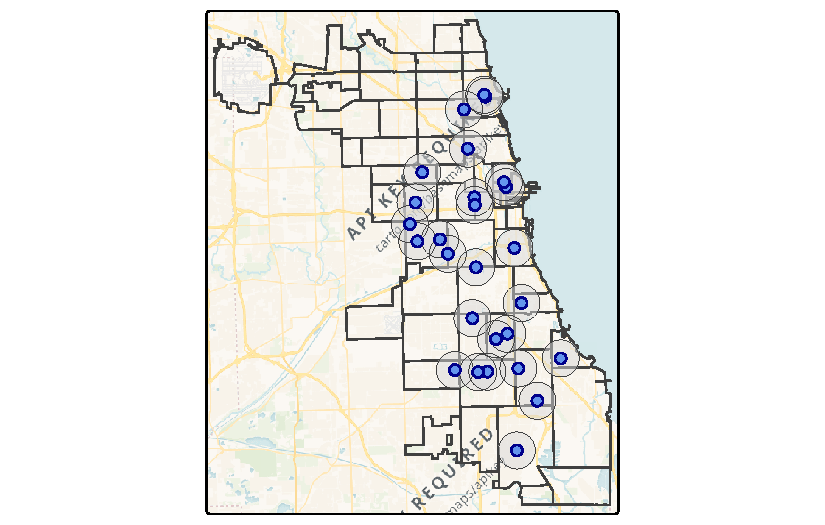
\includegraphics[keepaspectratio]{buffers_files/figure-pdf/unnamed-chunk-12-1.pdf}}

While this map shows our buffers were calculated correctly, the default
settings make it difficult to view. To improve aesthetics we change the
transparency of zip code boundaries by adjusting the alpha level. We add
a fill to the buffers, and make it transparent. We increase the size of
the points.

\begin{Shaded}
\begin{Highlighting}[]
\FunctionTok{tm\_basemap}\NormalTok{(}\StringTok{"CartoDB.VoyagerNoLabels"}\NormalTok{) }\SpecialCharTok{+} \CommentTok{\#Add Basemap}
  
  \FunctionTok{tm\_shape}\NormalTok{(areas}\FloatTok{.3435}\NormalTok{) }\SpecialCharTok{+} \FunctionTok{tm\_borders}\NormalTok{() }\SpecialCharTok{+} \CommentTok{\#Include Borders only from Areas}

  \FunctionTok{tm\_shape}\NormalTok{(metClinic\_buffers) }\SpecialCharTok{+} \FunctionTok{tm\_borders}\NormalTok{(}\AttributeTok{alpha =} \FloatTok{0.5}\NormalTok{, }\CommentTok{\#Slightly transparent }
                                           \AttributeTok{lwd =} \FloatTok{0.5}\NormalTok{) }\SpecialCharTok{+} \CommentTok{\#Reduce line weight}
  
    \FunctionTok{tm\_shape}\NormalTok{(metClinics}\FloatTok{.3435}\NormalTok{) }\SpecialCharTok{+} \FunctionTok{tm\_symbols}\NormalTok{(}\AttributeTok{size =} \FloatTok{0.5}\NormalTok{, }
                                    \AttributeTok{col=} \StringTok{"darkblue"}\NormalTok{, }
                                    \AttributeTok{fill=}\StringTok{"cornflowerblue"}\NormalTok{)}
\end{Highlighting}
\end{Shaded}

\pandocbounded{\includegraphics[keepaspectratio]{buffers_files/figure-pdf/unnamed-chunk-13-1.pdf}}

\subsection{Buffer union}\label{buffer-union}

While individual buffers are interesting and can be useful to consider
overlapping service areas, we are also interested in getting a sense of
which areas fall within a 1-mile service area in our study region -- or
not. For this, we need to to use a \textbf{union} spatial operation.
This will flatten all the individual buffers into one entity.

\begin{Shaded}
\begin{Highlighting}[]
\NormalTok{unionBuffers }\OtherTok{\textless{}{-}} \FunctionTok{st\_union}\NormalTok{(metClinic\_buffers)}
\end{Highlighting}
\end{Shaded}

Inspect the data structures of \texttt{metClinic\_buffers} and
\texttt{union.buffers} to see what happens to the data in this step.

Finally, we map the buffer union.

\begin{Shaded}
\begin{Highlighting}[]
\FunctionTok{tm\_basemap}\NormalTok{(}\StringTok{"CartoDB.VoyagerNoLabels"}\NormalTok{) }\SpecialCharTok{+} \CommentTok{\#Add Basemap}
  
  \FunctionTok{tm\_shape}\NormalTok{(areas}\FloatTok{.3435}\NormalTok{) }\SpecialCharTok{+} \FunctionTok{tm\_borders}\NormalTok{() }\SpecialCharTok{+} \CommentTok{\#Include Borders only from Areas}

  \FunctionTok{tm\_shape}\NormalTok{(unionBuffers) }\SpecialCharTok{+} \FunctionTok{tm\_borders}\NormalTok{(}\AttributeTok{alpha =} \FloatTok{0.8}\NormalTok{, }\CommentTok{\#Less transparent }
                                           \AttributeTok{lwd =} \FloatTok{0.5}\NormalTok{) }\SpecialCharTok{+} \CommentTok{\#Reduce line weight}
  
    \FunctionTok{tm\_shape}\NormalTok{(metClinics}\FloatTok{.3435}\NormalTok{) }\SpecialCharTok{+} \FunctionTok{tm\_symbols}\NormalTok{(}\AttributeTok{size =} \FloatTok{0.5}\NormalTok{, }
                                    \AttributeTok{col=} \StringTok{"darkblue"}\NormalTok{, }
                                    \AttributeTok{fill=}\StringTok{"cornflowerblue"}\NormalTok{)}
\end{Highlighting}
\end{Shaded}

\pandocbounded{\includegraphics[keepaspectratio]{buffers_files/figure-pdf/unnamed-chunk-15-1.pdf}}

\subsection{Save Data}\label{save-data-1}

We will save the merged 1-mile buffers to bring into maps for future
analysis. The \texttt{st\_write} function does the trick. Uncomment, and
run on your system!

\begin{Shaded}
\begin{Highlighting}[]
\CommentTok{\#st\_write(unionBuffers, "data/methadoneClinics\_1mi.shp")}
\end{Highlighting}
\end{Shaded}

\section{Rinse \& Repeat}\label{rinse-repeat}

From here, we can generate additional buffers to compare access
associations and generate multiple visuals.

We generate a two-mile buffer to add:

\begin{Shaded}
\begin{Highlighting}[]
\NormalTok{metClinic\_2mbuffers }\OtherTok{\textless{}{-}} \FunctionTok{st\_buffer}\NormalTok{(metClinics}\FloatTok{.3435}\NormalTok{, }\DecValTok{10560}\NormalTok{)}
\end{Highlighting}
\end{Shaded}

\subsection{Explore Cartographic
Styles}\label{explore-cartographic-styles}

And then, leverage tmap parameter specifications to further customize
the a map showing multiple buffers. We adjust the transparency of the
buffer fills, use different colors, and adjust borders to make the
visuals pop. Have fun in trying out new combinations!

We use the \texttt{tmap\_layout} function to take away the frame, add
and position a title. Explore the \texttt{tmap} documentation further to
find additional options for legends and more. To find color options in
R, there are multiple guides online (like
\href{https://bookdown.org/hneth/ds4psy/D-2-apx-colors-essentials.html}{this}
one).

\begin{Shaded}
\begin{Highlighting}[]
  \FunctionTok{tm\_shape}\NormalTok{(areas}\FloatTok{.3435}\NormalTok{) }\SpecialCharTok{+} \FunctionTok{tm\_borders}\NormalTok{() }\SpecialCharTok{+} 

  \FunctionTok{tm\_shape}\NormalTok{(metClinic\_2mbuffers) }\SpecialCharTok{+} \FunctionTok{tm\_polygons}\NormalTok{(}\AttributeTok{alpha =} \FloatTok{0.2}\NormalTok{,  }
                                           \AttributeTok{fill =} \StringTok{"darkgray"}\NormalTok{,}
                                           \AttributeTok{lwd =} \FloatTok{0.1}\NormalTok{) }\SpecialCharTok{+}
  
  \FunctionTok{tm\_shape}\NormalTok{(metClinic\_buffers) }\SpecialCharTok{+} \FunctionTok{tm\_polygons}\NormalTok{(}\AttributeTok{alpha =} \FloatTok{0.5}\NormalTok{, }
                                            \AttributeTok{fill =} \StringTok{"snow3"}\NormalTok{,}
                                           \AttributeTok{lwd =} \FloatTok{0.2}\NormalTok{) }\SpecialCharTok{+} \CommentTok{\#Reduce line weight + }
  
    \FunctionTok{tm\_shape}\NormalTok{(metClinics}\FloatTok{.3435}\NormalTok{) }\SpecialCharTok{+} \FunctionTok{tm\_symbols}\NormalTok{(}\AttributeTok{size =} \FloatTok{0.6}\NormalTok{, }
                                    \AttributeTok{col =} \StringTok{"aquamarine"}\NormalTok{,}
                                    \AttributeTok{fill=}\StringTok{"cornflowerblue"}\NormalTok{) }\SpecialCharTok{+} 
  
  \FunctionTok{tm\_layout}\NormalTok{(}\AttributeTok{main.title =} \StringTok{"Methadone Clinic Service Areas"}\NormalTok{,}
            \AttributeTok{main.title.position =} \StringTok{"center"}\NormalTok{,}
            \AttributeTok{frame =} \ConstantTok{FALSE}\NormalTok{)}
\end{Highlighting}
\end{Shaded}

\pandocbounded{\includegraphics[keepaspectratio]{buffers_files/figure-pdf/unnamed-chunk-18-1.pdf}}

Next, we'll try an interactive map to better explore the data that we
have. We switch the \texttt{tmap\_mode} to ``view'' and focus on our
buffer service areas, trying out a new color palette. We add labels for
zip codes using the \texttt{tm\_text} parameter. The resulting map lets
us zoom and out to explore the data. Clicking on a point will give
additional details about the Methadone provider.

\begin{Shaded}
\begin{Highlighting}[]
\CommentTok{\#tmap\_mode("view")}

\CommentTok{\#tm\_shape(areas.3435) + tm\_borders() + tm\_labels(text="zip") + }
  
\CommentTok{\#  tm\_shape(metClinic\_2mbuffers) + tm\_polygons(col = "darkmagenta",}
\CommentTok{\#                                              alpha = 0.2, lwd = 0) + }
  
\CommentTok{\#    tm\_shape(metClinic\_buffers) + tm\_polygons(col = "darkorchid4",}
\CommentTok{\#                                              alpha = 0.5, lwd = 0) +}
  
\CommentTok{\#    tm\_shape(metClinics.3435) + tm\_symbols(size = 0.5, fill="aquamarine3")}
\end{Highlighting}
\end{Shaded}

Which zip codes are within two miles walking distance to providers?
Which areas have the best coverage, versus the most challenging? In
future workshops, we'll learn how to take this visualization to the next
stage, by operationalizing a new variable per area. That could mean
calculating total buffer intersections per area, distance from the zip
code's center to the nearest resource, calculating area covered by
buffers, and more.

\bookmarksetup{startatroot}

\chapter{Link Community Data}\label{link-community-data}

\section{Overview}\label{overview-1}

Geographic location can serve as a ``key'' that links different datasets
together. By referencing each dataset and enabling its spatial location,
we can \textbf{integrate different types of information} in one setting.
In this tutorial, we will use the approximated ``service areas''
generated in our buffer analysis to identify vulnerable populations
during the COVID pandemic. We will connect Chicago COVID-19 Case data by
ZIP Code, available as a flat file on the
\href{https://data.cityofchicago.org/Health-Human-Services/COVID-19-Cases-Tests-and-Deaths-by-ZIP-Code/yhhz-zm2v}{city's
data portal}, to our environment.

We will then overlap the 1-mile buffers representing walkable access to
the Methadone providers in the city. We use a conservative threshold
because of the multiple challenges posed by the COVID pandemic that may
impact travel.

Our final goal will be to identify zip codes most impacted by COVID that
are outside our acceptable access threshold. Our tutorial objectives are
to:

\begin{itemize}
\tightlist
\item
  Clean data in preparation of merge
\item
  Integrate data using geographic identifiers
\item
  Generate maps for a basic gap analysis
\end{itemize}

\section{Environment Setup}\label{environment-setup}

To replicate the codes \& functions illustrated in this tutorial, you'll
need to have R and RStudio downloaded and installed on your system. This
tutorial assumes some familiarity with the R programming language.

\subsection{Input/Output}\label{BA-i-o}

Our inputs include multiple CSV and SHP files, all of which can be found
\href{https://github.com/GeoDaCenter/opioid-environment-toolkit/tree/master/data}{here},
though the providers point file was generated in the Geocoding tutorial.
Note that all four files are required (.dbf, .prj, .shp, and .shx) to
constitute a shapefile.

\begin{itemize}
\tightlist
\item
  Chicago Methadone Clinics, \texttt{methadone\_clinics.shp}
\item
  1-mile buffer zone of Clinics, \texttt{methadoneClinics\_1mi.shp}
\item
  Chicago Zip Codes, \texttt{Chicago\_Zips.shp}
\item
  Chicago COVID case data by Zip,
  \texttt{COVID-19\_Cases\_\_Tests\_\_and\_Deaths\_by\_ZIP\_Code.csv}
\end{itemize}

We will calculate the minimum distance between the resources and the
centroids of the zip codes, then save the results as a shapefile and as
a CSV. Our final result will be a shapefile/CSV with the minimum
distance value for each zip.

\subsection{Load Libraries}\label{load-libraries-1}

We will use the following packages in this tutorial:

\begin{itemize}
\tightlist
\item
  \texttt{sf}: to manipulate spatial data
\item
  \texttt{tmap}: to visualize and create maps
\item
  \texttt{units}: to convert units within spatial data
\end{itemize}

Load the libraries for use.

\begin{Shaded}
\begin{Highlighting}[]
\FunctionTok{library}\NormalTok{(sf)}
\FunctionTok{library}\NormalTok{(tmap)}
\end{Highlighting}
\end{Shaded}

\subsection{Load data}\label{load-data-2}

First we'll load the shapefiles.

\begin{Shaded}
\begin{Highlighting}[]
\NormalTok{chicagoZips }\OtherTok{\textless{}{-}} \FunctionTok{st\_read}\NormalTok{(}\StringTok{"data/Chicago\_Zips.shp"}\NormalTok{)}
\end{Highlighting}
\end{Shaded}

\begin{verbatim}
Reading layer `Chicago_Zips' from data source 
  `/Users/maryniakolak/Code/opioid-environment-toolkit/data/Chicago_Zips.shp' 
  using driver `ESRI Shapefile'
Simple feature collection with 61 features and 4 fields
Geometry type: MULTIPOLYGON
Dimension:     XY
Bounding box:  xmin: -87.94011 ymin: 41.64454 xmax: -87.52414 ymax: 42.02304
Geodetic CRS:  WGS84(DD)
\end{verbatim}

\begin{Shaded}
\begin{Highlighting}[]
\NormalTok{methadoneSf }\OtherTok{\textless{}{-}} \FunctionTok{st\_read}\NormalTok{(}\StringTok{"data/methadone\_clinics.shp"}\NormalTok{)}
\end{Highlighting}
\end{Shaded}

\begin{verbatim}
Reading layer `methadone_clinics' from data source 
  `/Users/maryniakolak/Code/opioid-environment-toolkit/data/methadone_clinics.shp' 
  using driver `ESRI Shapefile'
Simple feature collection with 27 features and 8 fields
Geometry type: POINT
Dimension:     XY
Bounding box:  xmin: -87.7349 ymin: 41.68698 xmax: -87.57673 ymax: 41.96475
Geodetic CRS:  WGS 84
\end{verbatim}

\begin{Shaded}
\begin{Highlighting}[]
\NormalTok{buffers}\OtherTok{\textless{}{-}} \FunctionTok{st\_read}\NormalTok{(}\StringTok{"data/methadoneClinics\_1mi.shp"}\NormalTok{)}
\end{Highlighting}
\end{Shaded}

\begin{verbatim}
Reading layer `methadoneClinics_1mi' from data source 
  `/Users/maryniakolak/Code/opioid-environment-toolkit/data/methadoneClinics_1mi.shp' 
  using driver `ESRI Shapefile'
Simple feature collection with 1 feature and 1 field
Geometry type: MULTIPOLYGON
Dimension:     XY
Bounding box:  xmin: 1141979 ymin: 1824050 xmax: 1195960 ymax: 1935751
Projected CRS: NAD83 / Illinois East (ftUS)
\end{verbatim}

Next, we'll load some new data we're interested in joining in: Chicago
COVID-19 Cases, Tests, and Deaths by ZIP Code, found on the city data
portal
\href{https://data.cityofchicago.org/Health-Human-Services/COVID-19-Cases-Tests-and-Deaths-by-ZIP-Code/yhhz-zm2v}{here}.
We'll load in a CSV and inspect the data:

\begin{Shaded}
\begin{Highlighting}[]
\NormalTok{COVID }\OtherTok{\textless{}{-}} \FunctionTok{read.csv}\NormalTok{(}\StringTok{"data/COVID{-}19\_Cases\_\_Tests\_\_and\_Deaths\_by\_ZIP\_Code.csv"}\NormalTok{)}
\end{Highlighting}
\end{Shaded}

\section{Inspect Data}\label{inspect-data}

\subsection{Identify Geographic Key}\label{identify-geographic-key}

The spatial zip dataset will be our primary file. We we need to first
identify the \textbf{geographic identifier} we would like to merge on.
What is the main key of interest that we will merge our data on?

\begin{Shaded}
\begin{Highlighting}[]
\FunctionTok{head}\NormalTok{(chicagoZips)}
\end{Highlighting}
\end{Shaded}

\begin{verbatim}
Simple feature collection with 6 features and 4 fields
Geometry type: MULTIPOLYGON
Dimension:     XY
Bounding box:  xmin: -87.80649 ymin: 41.88747 xmax: -87.59852 ymax: 41.93228
Geodetic CRS:  WGS84(DD)
  objectid shape_area shape_len   zip                       geometry
1       33  106052287  42720.04 60647 MULTIPOLYGON (((-87.67762 4...
2       34  127476051  48103.78 60639 MULTIPOLYGON (((-87.72683 4...
3       35   45069038  27288.61 60707 MULTIPOLYGON (((-87.785 41....
4       36   70853834  42527.99 60622 MULTIPOLYGON (((-87.66707 4...
5       37   99039621  47970.14 60651 MULTIPOLYGON (((-87.70656 4...
6       38   23506056  34689.35 60611 MULTIPOLYGON (((-87.61401 4...
\end{verbatim}

In this dataset, we can see that the column showing our geographic key
is ``zip.''

\subsection{Inspect Case Data}\label{inspect-case-data}

Next, let's inspect COVID case data. What information do we need from
this file? We may not need everything, so consider just identifying the
field with the geographic identifier and main variable(s) of interest.

\begin{Shaded}
\begin{Highlighting}[]
\FunctionTok{head}\NormalTok{(COVID)}
\end{Highlighting}
\end{Shaded}

\begin{verbatim}
  ZIP.Code Week.Number Week.Start   Week.End Cases...Weekly Cases...Cumulative
1    60603          39 09/20/2020 09/26/2020              0                 13
2    60604          39 09/20/2020 09/26/2020              0                 31
3    60611          16 04/12/2020 04/18/2020              8                 72
4    60611          15 04/05/2020 04/11/2020              7                 64
5    60615          11 03/08/2020 03/14/2020             NA                 NA
6    60603          10 03/01/2020 03/07/2020             NA                 NA
  Case.Rate...Weekly Case.Rate...Cumulative Tests...Weekly Tests...Cumulative
1                  0                 1107.3             25                327
2                  0                 3964.2             12                339
3                 25                  222.0            101                450
4                 22                  197.4             59                349
5                 NA                     NA              6                  9
6                 NA                     NA              0                  0
  Test.Rate...Weekly Test.Rate...Cumulative Percent.Tested.Positive...Weekly
1               2130                27853.5                              0.0
2               1534                43350.4                              0.0
3                312                 1387.8                              0.1
4                182                 1076.3                              0.1
5                 14                   21.7                               NA
6                  0                    0.0                               NA
  Percent.Tested.Positive...Cumulative Deaths...Weekly Deaths...Cumulative
1                                  0.0               0                   0
2                                  0.1               0                   0
3                                  0.2               0                   0
4                                  0.2               0                   0
5                                   NA               0                   0
6                                   NA               0                   0
  Death.Rate...Weekly Death.Rate...Cumulative Population   Row.ID
1                   0                       0       1174 60603-39
2                   0                       0        782 60604-39
3                   0                       0      32426 60611-16
4                   0                       0      32426 60611-15
5                   0                       0      41563 60615-11
6                   0                       0       1174 60603-10
             ZIP.Code.Location
1 POINT (-87.625473 41.880112)
2 POINT (-87.629029 41.878153)
3 POINT (-87.620291 41.894734)
4 POINT (-87.620291 41.894734)
5 POINT (-87.602725 41.801993)
6 POINT (-87.625473 41.880112)
\end{verbatim}

From this we can assess the need for the following variables: ZIP Code
and Percent Tested Positive - Cumulative. Let's subset the data
accordingly. Because this data file has extremely long header names
(common in the epi world), let's use the \texttt{colnames} function to
get exactly what we need.

\begin{Shaded}
\begin{Highlighting}[]
\FunctionTok{colnames}\NormalTok{(COVID)}
\end{Highlighting}
\end{Shaded}

\begin{verbatim}
 [1] "ZIP.Code"                            
 [2] "Week.Number"                         
 [3] "Week.Start"                          
 [4] "Week.End"                            
 [5] "Cases...Weekly"                      
 [6] "Cases...Cumulative"                  
 [7] "Case.Rate...Weekly"                  
 [8] "Case.Rate...Cumulative"              
 [9] "Tests...Weekly"                      
[10] "Tests...Cumulative"                  
[11] "Test.Rate...Weekly"                  
[12] "Test.Rate...Cumulative"              
[13] "Percent.Tested.Positive...Weekly"    
[14] "Percent.Tested.Positive...Cumulative"
[15] "Deaths...Weekly"                     
[16] "Deaths...Cumulative"                 
[17] "Death.Rate...Weekly"                 
[18] "Death.Rate...Cumulative"             
[19] "Population"                          
[20] "Row.ID"                              
[21] "ZIP.Code.Location"                   
\end{verbatim}

\subsection{Subset Data}\label{subset-data}

We can now subset to just include the fields we need. There are many
different ways to subset in R -- we just use one example here! Inspect
your data to confirm it was pulled correctly.

\begin{Shaded}
\begin{Highlighting}[]
\FunctionTok{library}\NormalTok{(dplyr)}
\end{Highlighting}
\end{Shaded}

\begin{verbatim}

Attaching package: 'dplyr'
\end{verbatim}

\begin{verbatim}
The following objects are masked from 'package:stats':

    filter, lag
\end{verbatim}

\begin{verbatim}
The following objects are masked from 'package:base':

    intersect, setdiff, setequal, union
\end{verbatim}

\begin{Shaded}
\begin{Highlighting}[]
\NormalTok{COVID.sub19 }\OtherTok{\textless{}{-}}\NormalTok{ COVID }\SpecialCharTok{\%\textgreater{}\%}
    \FunctionTok{filter}\NormalTok{(Week.Number }\SpecialCharTok{==} \DecValTok{19}\NormalTok{) }\SpecialCharTok{\%\textgreater{}\%}
    \FunctionTok{select}\NormalTok{(ZIP.Code,Case.Rate...Cumulative)}

\NormalTok{COVID.sub39 }\OtherTok{\textless{}{-}}\NormalTok{ COVID }\SpecialCharTok{\%\textgreater{}\%}
    \FunctionTok{filter}\NormalTok{(Week.Number }\SpecialCharTok{==} \DecValTok{39}\NormalTok{) }\SpecialCharTok{\%\textgreater{}\%}
    \FunctionTok{select}\NormalTok{(ZIP.Code,Case.Rate...Cumulative)}

\FunctionTok{glimpse}\NormalTok{(COVID.sub19)}
\end{Highlighting}
\end{Shaded}

\begin{verbatim}
Rows: 60
Columns: 2
$ ZIP.Code               <chr> "60604", "60601", "60612", "60613", "60615", "6~
$ Case.Rate...Cumulative <dbl> 1790.3, 429.3, 1468.9, 628.6, 659.2, 541.4, 175~
\end{verbatim}

\begin{Shaded}
\begin{Highlighting}[]
\FunctionTok{colnames}\NormalTok{(COVID.sub19) }\OtherTok{\textless{}{-}} \FunctionTok{c}\NormalTok{(}\StringTok{"zip"}\NormalTok{, }\StringTok{"CaseRtWk19"}\NormalTok{)}
\FunctionTok{colnames}\NormalTok{(COVID.sub39) }\OtherTok{\textless{}{-}} \FunctionTok{c}\NormalTok{(}\StringTok{"zip"}\NormalTok{, }\StringTok{"CaseRtWk39"}\NormalTok{)}
\end{Highlighting}
\end{Shaded}

\section{Merge Data}\label{merge-data}

Let's merge the data using the zip code geographic identifier, ``ZIP
Code'' field, to bring in the the Percent Tested Positive - Cumalative
dataset. Inspect the data to confirm it merged correctly!

\begin{Shaded}
\begin{Highlighting}[]
\FunctionTok{dim}\NormalTok{(chicagoZips)}
\end{Highlighting}
\end{Shaded}

\begin{verbatim}
[1] 61  5
\end{verbatim}

\begin{Shaded}
\begin{Highlighting}[]
\NormalTok{zipsMerged }\OtherTok{\textless{}{-}} \FunctionTok{merge}\NormalTok{(chicagoZips, COVID.sub19, }\AttributeTok{by =} \StringTok{"zip"}\NormalTok{, }\AttributeTok{all.x =} \ConstantTok{TRUE}\NormalTok{)}

\FunctionTok{head}\NormalTok{(zipsMerged)}
\end{Highlighting}
\end{Shaded}

\begin{verbatim}
Simple feature collection with 6 features and 5 fields
Geometry type: MULTIPOLYGON
Dimension:     XY
Bounding box:  xmin: -87.63999 ymin: 41.85317 xmax: -87.60246 ymax: 41.88913
Geodetic CRS:  WGS84(DD)
    zip objectid shape_area shape_len CaseRtWk19                       geometry
1 60601       27    9166246  19804.58      429.3 MULTIPOLYGON (((-87.62271 4...
2 60602       26    4847125  14448.17      643.1 MULTIPOLYGON (((-87.60997 4...
3 60603       19    4560229  13672.68         NA MULTIPOLYGON (((-87.61633 4...
4 60604       48    4294902  12245.81     1790.3 MULTIPOLYGON (((-87.63376 4...
5 60605       20   36301276  37973.35      541.4 MULTIPOLYGON (((-87.62064 4...
6 60606       31    6766411  12040.44      612.7 MULTIPOLYGON (((-87.63397 4...
\end{verbatim}

\begin{Shaded}
\begin{Highlighting}[]
\NormalTok{zipsMerged }\OtherTok{\textless{}{-}} \FunctionTok{merge}\NormalTok{(zipsMerged, COVID.sub39, }\AttributeTok{by =} \StringTok{"zip"}\NormalTok{, }\AttributeTok{all.x =} \ConstantTok{TRUE}\NormalTok{)}
\FunctionTok{head}\NormalTok{(zipsMerged)}
\end{Highlighting}
\end{Shaded}

\begin{verbatim}
Simple feature collection with 6 features and 6 fields
Geometry type: MULTIPOLYGON
Dimension:     XY
Bounding box:  xmin: -87.63999 ymin: 41.85317 xmax: -87.60246 ymax: 41.88913
Geodetic CRS:  WGS84(DD)
    zip objectid shape_area shape_len CaseRtWk19 CaseRtWk39
1 60601       27    9166246  19804.58      429.3     1451.4
2 60602       26    4847125  14448.17      643.1     1688.1
3 60603       19    4560229  13672.68         NA     1107.3
4 60604       48    4294902  12245.81     1790.3     3964.2
5 60605       20   36301276  37973.35      541.4     1420.8
6 60606       31    6766411  12040.44      612.7     2289.6
                        geometry
1 MULTIPOLYGON (((-87.62271 4...
2 MULTIPOLYGON (((-87.60997 4...
3 MULTIPOLYGON (((-87.61633 4...
4 MULTIPOLYGON (((-87.63376 4...
5 MULTIPOLYGON (((-87.62064 4...
6 MULTIPOLYGON (((-87.63397 4...
\end{verbatim}

\section{Visualize Data}\label{visualize-data}

Now we are ready to visualize our data! First we'll make a simple map.
We generate a choropleth map of case rate data using quantile bins, and
the Blue-Purple color palette. You can find an R color cheatsheet useful
for identifying palette codes
\href{https://www.nceas.ucsb.edu/sites/default/files/2020-04/colorPaletteCheatsheet.pdf}{here}.
(More details on thematic mapping are in tutorials that follow!) We
overlay the buffers and clincal providers.

\begin{Shaded}
\begin{Highlighting}[]
\FunctionTok{tm\_shape}\NormalTok{(zipsMerged) }\SpecialCharTok{+}
  \FunctionTok{tm\_polygons}\NormalTok{(}\AttributeTok{col =} \StringTok{"CaseRtWk39"}\NormalTok{, }
              \AttributeTok{palette =}\StringTok{"BuPu"}\NormalTok{,}
              \AttributeTok{style =} \StringTok{"jenks"}\NormalTok{,}
              \AttributeTok{title =} \StringTok{"COVID Case Rate"}\NormalTok{) }\SpecialCharTok{+}
  
  \FunctionTok{tm\_shape}\NormalTok{(buffers) }\SpecialCharTok{+} \FunctionTok{tm\_borders}\NormalTok{() }\SpecialCharTok{+}
  \FunctionTok{tm\_shape}\NormalTok{(methadoneSf) }\SpecialCharTok{+} \FunctionTok{tm\_dots}\NormalTok{(}\AttributeTok{size =} \FloatTok{0.3}\NormalTok{) }
\end{Highlighting}
\end{Shaded}

\begin{verbatim}
\end{verbatim}

\begin{verbatim}
-- tmap v3 code detected -------------------------------------------------------
\end{verbatim}

\begin{verbatim}
[v3->v4] `tm_polygons()`: instead of `style = "jenks"`, use fill.scale =
`tm_scale_intervals()`.
i Migrate the argument(s) 'style', 'palette' (rename to 'values') to
  'tm_scale_intervals(<HERE>)'
[v3->v4] `tm_polygons()`: use 'fill' for the fill color of polygons/symbols
(instead of 'col'), and 'col' for the outlines (instead of 'border.col').
[v3->v4] `tm_polygons()`: migrate the argument(s) related to the legend of the
visual variable `fill` namely 'title' to 'fill.legend = tm_legend(<HERE>)'
[cols4all] color palettes: use palettes from the R package cols4all. Run
`cols4all::c4a_gui()` to explore them. The old palette name "BuPu" is named
"brewer.bu_pu"
Multiple palettes called "bu_pu" found: "brewer.bu_pu", "matplotlib.bu_pu". The first one, "brewer.bu_pu", is returned.
\end{verbatim}

\pandocbounded{
\includegraphics[keepaspectratio]{linking_files/figure-pdf/unnamed-chunk-8-1.pdf}}

Already we can generate some insight. Areas on the far West side of the
city have some of the highest case rates, but are outside a walkable
distance to Methadone providers. For individuals with opioid use
disorder requiring medication access in these locales, they may be
especially vulnerable during the pandemic.

Next, we adjust some \texttt{tmap} parameters to improve our map. Now we
switch to a red-yellow-green palette, and specify six bins for our
quantile map. We flip the direction of the palette using a negative
sign, so that red corresponds to areas with higher rates. We adjust
transparency using an \texttt{alpha} parameter, and line thickness using
the \texttt{lwd} parameter.

\begin{Shaded}
\begin{Highlighting}[]
\NormalTok{wk19 }\OtherTok{=} \FunctionTok{tm\_shape}\NormalTok{(zipsMerged) }\SpecialCharTok{+}
  \FunctionTok{tm\_polygons}\NormalTok{(}\AttributeTok{col =} \StringTok{"CaseRtWk19"}\NormalTok{, }
              \AttributeTok{palette =}\StringTok{"BuPu"}\NormalTok{,}
              \AttributeTok{breaks =} \FunctionTok{c}\NormalTok{(}\DecValTok{1000}\NormalTok{,}\DecValTok{2000}\NormalTok{,}\DecValTok{3000}\NormalTok{,}\DecValTok{4000}\NormalTok{,}\DecValTok{5000}\NormalTok{),}
              \AttributeTok{title =} \StringTok{"COVID Case Rate"}\NormalTok{) }\SpecialCharTok{+}

  \FunctionTok{tm\_shape}\NormalTok{(buffers) }\SpecialCharTok{+} \FunctionTok{tm\_borders}\NormalTok{(}\AttributeTok{col =} \StringTok{"white"}\NormalTok{) }\SpecialCharTok{+} \FunctionTok{tm\_fill}\NormalTok{(}\AttributeTok{alpha=}\FloatTok{0.5}\NormalTok{) }\SpecialCharTok{+}
  \FunctionTok{tm\_shape}\NormalTok{(methadoneSf) }\SpecialCharTok{+} \FunctionTok{tm\_dots}\NormalTok{(}\AttributeTok{col =} \StringTok{"white"}\NormalTok{, }\AttributeTok{size =} \FloatTok{0.3}\NormalTok{) }\SpecialCharTok{+}
  \FunctionTok{tm\_layout}\NormalTok{(}\AttributeTok{scale =} \FloatTok{0.7}\NormalTok{,}
            \AttributeTok{main.title =} \StringTok{"Walkable Methadone Service Areas in Week 19"}\NormalTok{,}
            \AttributeTok{main.title.position =} \StringTok{"center"}\NormalTok{,}
            \AttributeTok{main.title.size =} \DecValTok{1}\NormalTok{,}
            \AttributeTok{frame.lwd =} \DecValTok{0}\NormalTok{)}

\NormalTok{wk39 }\OtherTok{\textless{}{-}} \FunctionTok{tm\_shape}\NormalTok{(zipsMerged) }\SpecialCharTok{+}
  \FunctionTok{tm\_polygons}\NormalTok{(}\AttributeTok{col =} \StringTok{"CaseRtWk39"}\NormalTok{, }
              \AttributeTok{palette =}\StringTok{"BuPu"}\NormalTok{,}
              \AttributeTok{breaks =} \FunctionTok{c}\NormalTok{(}\DecValTok{1000}\NormalTok{,}\DecValTok{2000}\NormalTok{,}\DecValTok{3000}\NormalTok{,}\DecValTok{4000}\NormalTok{,}\DecValTok{5000}\NormalTok{),}
              \AttributeTok{title =} \StringTok{"COVID Case Rate"}\NormalTok{) }\SpecialCharTok{+}
  \FunctionTok{tm\_borders}\NormalTok{(}\AttributeTok{lwd =} \DecValTok{0}\NormalTok{) }\SpecialCharTok{+} 
  \FunctionTok{tm\_shape}\NormalTok{(buffers) }\SpecialCharTok{+} \FunctionTok{tm\_borders}\NormalTok{(}\AttributeTok{col =} \StringTok{"white"}\NormalTok{) }\SpecialCharTok{+} \FunctionTok{tm\_fill}\NormalTok{(}\AttributeTok{alpha=}\FloatTok{0.5}\NormalTok{) }\SpecialCharTok{+}
  \FunctionTok{tm\_shape}\NormalTok{(methadoneSf) }\SpecialCharTok{+} \FunctionTok{tm\_dots}\NormalTok{(}\AttributeTok{col =} \StringTok{"white"}\NormalTok{, }\AttributeTok{size =} \FloatTok{0.3}\NormalTok{) }\SpecialCharTok{+}
  \FunctionTok{tm\_legend}\NormalTok{(}\AttributeTok{orientation =} \StringTok{"landscape"}\NormalTok{) }\SpecialCharTok{+} 
  \FunctionTok{tm\_layout}\NormalTok{(}\AttributeTok{main.title =} \StringTok{"Walkable Methadone Service Areas in Week 39"}\NormalTok{,}
            \AttributeTok{main.title.position =} \StringTok{"center"}\NormalTok{,}
            \AttributeTok{main.title.size =} \DecValTok{1}\NormalTok{,}
            \AttributeTok{frame.alpha =} \FloatTok{0.5}\NormalTok{)}

\FunctionTok{tmap\_arrange}\NormalTok{(wk19,wk39)}
\end{Highlighting}
\end{Shaded}

\pandocbounded{\includegraphics[keepaspectratio]{linking_files/figure-pdf/unnamed-chunk-9-1.pdf}}

Run the same code with a dynamic map! As done previously, change the
\texttt{tmap\_mode} to ``view'' and zoom in to view specific zip codes.

Using this approach, it's clear that the zip codes on the West Side most
vulnerable are 60651, 60644, 60632, 60629, and 60608. By updating the
thresholds and parameters further, these can shift as well to be more or
less conservative based on our assumptions.

\subsection{Save Data}\label{save-data-2}

We save our newly merged ZCTA level data for future analysis.

\begin{Shaded}
\begin{Highlighting}[]
\CommentTok{\#write\_sf(zipsMerged, "data/chizips\_COVID.gpkg")}
\end{Highlighting}
\end{Shaded}

\bookmarksetup{startatroot}

\chapter*{References}\label{references}
\addcontentsline{toc}{chapter}{References}

\markboth{References}{References}

\phantomsection\label{refs}




\end{document}
